\documentclass[a4paper,UKenglish,cleveref, autoref, thm-restate, screen]{lipics-v2021}

\pdfoutput=1 %uncomment to ensure pdflatex processing (mandatatory e.g. to submit to arXiv)
\hideLIPIcs  %uncomment to remove references to LIPIcs series (logo, DOI, ...), e.g. when preparing a pre-final version to be uploaded to arXiv or another public repository

%\graphicspath{{./graphics/}}%helpful if your graphic files are in another directory


\title{From Tarski to Russell : Bridging Explicit and Implicit presentations of Type Theory}

%\titlerunning{Dummy short title} 

\author{Thierry Coquand}{Chalmers University of Technology -- University of Gothenburg, Sweden}{coquand@chalmers.se}{https://orcid.org/0000-0002-5429-5153}{}

\author{Raphaël Sterbac}{ENS Paris-Saclay -- Université Paris-Saclay, France}{raphael.sterbac@ens-paris-saclay.fr}{https://orcid.org/0009-0001-6779-8323}{}

\authorrunning{T. Coquand and R. Sterbac} 

\Copyright{Thierry Coquand and Raphaël Sterbac} 

\ccsdesc[500]{Theory of computation~Type theory}

\keywords{Type theory, Universes, Cumulativity} 

\category{} %optional, e.g. invited paper

\relatedversion{} %optional, e.g. full version hosted on arXiv, HAL, or other respository/website
%\relatedversiondetails[linktext={opt. text shown instead of the URL}, cite=DBLP:books/mk/GrayR93]{Classification (e.g. Full Version, Extended Version, Previous Version}{URL to related version} %linktext and cite are optional

%\supplement{}%optional, e.g. related research data, source code, ... hosted on a repository like zenodo, figshare, GitHub, ...
%\supplementdetails[linktext={opt. text shown instead of the URL}, cite=DBLP:books/mk/GrayR93, subcategory={Description, Subcategory}, swhid={Software Heritage Identifier}]{General Classification (e.g. Software, Dataset, Model, ...)}{URL to related version} %linktext, cite, and subcategory are optional

%\funding{(Optional) general funding statement \dots}%optional, to capture a funding statement, which applies to all authors. Please enter author specific funding statements as fifth argument of the \author macro.


\nolinenumbers %uncomment to disable line numbering



%Editor-only macros:: begin (do not touch as author)%%%%%%%%%%%%%%%%%%%%%%%%%%%%%%%%%%
\EventEditors{John Q. Open and Joan R. Access}
\EventNoEds{2}
\EventLongTitle{42nd Conference on Very Important Topics (CVIT 2016)}
\EventShortTitle{CVIT 2016}
\EventAcronym{CVIT}
\EventYear{2016}
\EventDate{December 24--27, 2016}
\EventLocation{Little Whinging, United Kingdom}
\EventLogo{}
\SeriesVolume{42}
\ArticleNo{23}
%%%%%%%%%%%%%%%%%%%%%%%%%%%%%%%%%%%%%%%%%%%%%%%%%%%%%%

\usepackage{ebproof}
\usepackage{ebproof-rules}
\usepackage{mathpartir}
\usepackage{verbatim}
\usepackage{float}
\usepackage{circuitikz}
\usepackage{stmaryrd}

\usepackage[dvipsnames]{xcolor}
\definecolor{Bg}{HTML}{F9F9F9}
\usepackage{tcolorbox}
\tcbuselibrary{skins,breakable}
\newtcolorbox{rulebox}[1][]{
  enhanced,
  breakable,
  frame hidden,
  arc=2pt,
  outer arc=2pt,
  colframe=black,
  coltitle=black,
  detach title,
  before upper={\tcbtitle\par\vspace{1ex}},
  top=3pt,
  bottom=0pt,
  left=3pt,
  right=3pt,
  colback=Bg,
  #1
}
\usepackage{hyperref}
\hypersetup{
    colorlinks=true,
    linkcolor=black,
    filecolor=magenta,      
    urlcolor=Blue,
    citecolor=Green
}

\usepackage{tikz-cd}
\usepackage{amsthm}
\usepackage{amsmath}
\usepackage{amssymb} 

% Formatted letters
\newcommand{\bC}{\mathbb{C}}
\newcommand{\bR}{\mathbb{R}}
\newcommand{\bN}{\mathbb{N}}
\newcommand{\bZ}{\mathbb{Z}}
\newcommand{\bQ}{\mathbb{Q}}
\newcommand{\bK}{\mathbb{K}}
\newcommand{\bF}{\mathbb{F}}
\newcommand{\bM}{\mathbb{M}}
\newcommand{\bGL}{\mathbb{GL}}
\newcommand{\cC}{\mathcal{C}}
\newcommand{\cD}{\mathcal{D}}
\newcommand{\cO}{\mathcal{O}}


% Text command for text strings I need to type in math mode
\newcommand{\coe}{\mathsf{coe}}
\newcommand{\JoinTy}{\mathsf{Join}}
\newcommand{\nf}{\mathsf{nf}}
\newcommand{\ctx}{\mathsf{ctx}}
\newcommand{\reify}{\mathsf{reify}}
\newcommand{\Var}{\mathsf{Var}}
\newcommand{\Norm}{\mathsf{Norm}}
\newcommand{\Neut}{\mathsf{Neut}}
\newcommand{\Elem}{\mathsf{Tm}}
\newcommand{\Type}{\mathsf{Ty}}
\newcommand{\Term}{\mathsf{Term}}
\newcommand{\type}{\mathsf{type}}
\newcommand{\Set}{\mathsf{Set}}
\newcommand{\conv}{\mathsf{conv}}
\newcommand{\strip}{\mathsf{strip}}
\newcommand{\erase}{\mathsf{erase}}
\newcommand{\fold}{\mathsf{fold}}
\newcommand{\app}{\mathsf{app}}
\newcommand{\brec}{\mathsf{brec}}
\newcommand{\Id}{\mathsf{id}}
\newcommand{\p}{\mathsf{p}}
\newcommand{\q}{\mathsf{q}}
\newcommand{\lvq}{\mathsf{lq}}
\newcommand{\lvp}{\mathsf{lp}}
\newcommand{\lvid}{\mathsf{lid}}
\newcommand{\mk}{\mathsf{mk}}
\newcommand{\fst}{\mathsf{fst}}
\newcommand{\snd}{\mathsf{snd}}
\newcommand{\lst}{\mathsf{list}}
\renewcommand{\r}{\mathsf{r}}
\newcommand{\U}{\mathsf{U}}
\newcommand{\N}{\mathsf{N}}
\newcommand{\NA}{\mathsf{NA}}

\usepackage[square,numbers]{natbib}

\bibliographystyle{plainnat}

\ebproofset{
    rule margin=0.5ex,
    separation=1em
}
\NewDocumentEnvironment{mathparsmall}{}
  {%
    \small
    \begin{mathparpagebreakable}
  }
  {%
    \end{mathparpagebreakable}%
  }

\NewDocumentEnvironment{mathpartiny}{}
  {%
    \scriptsize
    \begin{mathparpagebreakable}
  }
  {%
    \end{mathparpagebreakable}%
  }

% Rocq links

\DeclareDocumentCommand{\coqlogo}{}{\raisebox{-.2em}{
\includegraphics[height=1em]{icon-rocq-blue-eps-converted-to.pdf}}}
\DeclareDocumentCommand{\formfile}{O{blob/8920605948f1c2d0b92fd81ace628cb6996f46fe/} m}{%
  \href{https://github.com/raphael-sterbac/Russell-Tarski-Equivalence/\IfValueT{#1}{#1}#2}{\coqlogo}}

\DeclareDocumentCommand{\formline}{O{blob/8920605948f1c2d0b92fd81ace628cb6996f46fe/} m m m}{%
  \href{https://github.com/raphael-sterbac/Russell-Tarski-Equivalence/\IfValueT{#1}{#1}#2\#L#3}{\coqlogo}}

\begin{document}

\maketitle

\begin{abstract}
    We present a modular and algorithmic proof for the equivalence of different
    presentations of type theory, notably relating Russell and Tarski presentations of cumulative
    universe hierarchies. More generally, we relate the generalised algebraic and pure type system formulations of the syntax, bridging
    the gap between the type theory used to prove metatheoretical results, and the one often used in practice.
    Our work can also be seen as an effort to extend initiality results to implicit presentations of type theory.
\end{abstract}


\section{Introduction}

In type theory, universes allow manipulating types as terms.
To avoid Girard's paradox, it is routine to introduce a \textit{hierarchy} of universes: $\U_0, \U_1, \U_2, ...$.
In practical systems, those are often assumed to be \textit{cumulative}, requiring proper inclusions between them.
There are two different ways to formulate the notion of universe in type theory. Martin-Löf’s
first versions \cite{MARTINLOF75, MARTINLOF82} were formulated à la Russell, where a universe is seen as a type of types. Later, an alternative version à la Tarski \cite{MARTINLOF84}, where a universe is seen as a type of codes along with a decoding function, was also introduced. Usually, Russell universes are regarded as an informal notation of the latter, as \cite{Luo} suggested.

When presenting Type Theory in an algebraic fashion, Tarski universes are essential, at least if we do not want to introduce sort equations, and one can show that the system à la Tarski presents the initial model of such a theory.
This initial model has been constructed explicitly in \citet{bcde2026}, following the method presented in \citet{Streicher} and formalised in \citet{Brunerie}. 
However, there are as many initiality theorems as there are presentations of type theory, and if people often assume that they
extend easily to the more informal syntax used in practice, this comes from misconceptions as they depend on subtle details of the presentation.
To solve this issue, Voevodsky proposed the \textit{Initiality Conjecture project}, which aimed at developing rigorous metatheory for large class of theories.
A first step at solving this goal was achieved by Streicher \cite{Streicher}, proving initiality for a fully annotated Calculus of Constructions, and then
proving its equivalence with the more common, unannotated formulation, close to a Pure Type System. 

Generalised Algebraic Theories (GATs) provide a framework to describe type theories and their model in a uniform
way, and to prove initiality rather easily \cite{noteGAT, Brunerie}, 
thus solving the first part of the problem. However, GATs give rise to a fully explicit and annotated presentation of type theory, which is inconvenient to work in.
Therefore, it would be essential to extend Streicher's equivalence results to relate Generalised Algebraic and Pure Type System presentations, where the latter is presented
with Russell universes and unannotated syntax.  This would justify rigorously the common practice of using informal syntax and Russell universes, as proposed by \citet{Luo},
and would legitimate interpreting such syntax in the usual models of type theory.
In particular, our work essentially relates the results proven on explicit type theories using semantic arguments, to the corresponding implicit theories implemented in proof systems.

\noindent
\textbf{Related work.} In recent work, Assaf and Thiré \cite{assaf,thire} show the equivalence between Russell and Tarski presentation of universes for the Calculus
of Constructions with $\beta$ as an external reduction. Nevertheless, it appeared that their proof was 
incorrect, and a new proof using the same technique was finally published by \citet{tiago-fscd}. Unfortunately, their arguments do not apply to
formulations of type theory with judgemental equality, and do not extend to $\eta$-equivalence. 
This legitimates the study of a new proof technique. 

In the present paper, we will not consider cumulativity with a structural sub-typing judgement $A \leq B$ \cite{assaf,thire,Luo, subtyping},
as it can lead to discrepancy between Russell and Tarski universes in a more general setting, as pointed out by Luo \cite{Luo}.
For instance, sub-typing breaks canonicity when adding inductive types, and does not hold for $\Pi$-types in the Set model, or it is at least unclear
depending on the encoding of application in the ambient set theory. 
Therefore, here we will study the simplest form of cumulativity that is possible.
Yet, structural sub-typing would provide a more convenient manipulation of universes in a practical proof
assistant. Notably, it simplifies greatly the use of algebraic hierarchies \cite{subtyping}.
The recent work of \citet{AdapTT} presents a general framework which would provide automatically the necessary
equations to solve the issues mentioned above. In any case, we believe that our work is orthogonal to such considerations,
and that our proof should extend to any system that handles structural sub-typing in a correct way.\\

\noindent
\textbf{Contributions.} In this paper we show the equivalence of Russell and Tarski universes by a method due to \citet{Streicher},
for Martin Löf's Type Theory with dependent products, cumulative universes and judgmental $\beta\eta$ equality.
Our proof is modular and adapts to more complicated type systems. For instance, it adapts to a theory with universe polymorphism and internal universe levels \cite{polymorphism}.
More generally, we relate the Generalised Algebraic presentation of type theory to the implicit, and unannotated presentation
inherited from Pure Type Systems. In particular, our result justifies the practice of working in implicit
syntax, while legitimating the interpretation of implicit systems in usual models of type theory, such as in Categories with Families.
More precisely, our result proves that those two presentations have the same models.

The main argument is as follows: there is a natural forgetful map from the Tarski to the
Russell presentation. We show that any Russell judgement can be lifted in a unique way
to a Tarski judgement, proving the syntactic equivalence of the two theories.
This work is done in section \ref{sectionT2T2'}.
We rely on well-known properties of the syntax : no-confusion and injectivity of type formers, which are sometimes refered to as \textit{definitional inversion}.
We only need them at the level of the generalised algebraic theory, and they will propagate along our equivalence results.
Those properties seem to be strongly related to conversion \cite{meven}, and our equivalence result itself is to be
related to the elaboration in proof assistants.

Our proof is elementary and provides an algorithm to translate from one presentation to the other. Notably,
we only rely on the basic induction principles for the syntax, and not on stronger induction principles given
by normalisation. The definitional inversion properties are proven using the new domain-theoretic technique of \citet{definitional-inv}. Thus we believe that our proof could be adapted to various theories which do not enjoy this property.
In fact, the proof is purely syntactic and can be done internal to a weak metatheory such as primitive recursive
arithmetic, whereas normalisation relies on a stronger metatheory \cite{Coq19} such as the constructive set theory of \citet{aczel}.

In addition, we manually formalised and verified our equivalence result between Tarski and Russell universes in Rocq \cite{Formalisation}.
Throughout the paper, we provide links to the corresponding definitions and theorems
in the formalisation, indicated by the Rocq logo 
\includegraphics[height=1em]{icon-rocq-blue-eps-converted-to.pdf}.
Along with this, we did a complete auto-formalisation in Agda of the whole paper using Claude \cite{auto-formalisation}.\\

\noindent
\textbf{Structure of this paper.}
In Section \ref{GAT} we present the fully explicit Generalised Algebraic Theory and prove definitional inversion, before presenting the zoo of implicit presentations in Section \ref{implicit-presentations}.
Then, we prove that all those syntaxes are equivalent in the following sections: 

\begin{itemize}
    \item[] \textbf{\S\S~\ref{sectionT0T1}.} We relate explicit and implicit substitutions. 
    \item[] \textbf{\S\S~\ref{sectionT1T2}.} We relate Tarski and Russell presentations for cumulative universes.
    \item[] \textbf{\S\S~\ref{sectionT2T2'}.} We relate annotated and unannotated syntaxes. 
\end{itemize}


\section{The Generalised Algebraic Theory and No-Confusion}\label{GAT}

\subsection{A fully explicit presentation}

In this section, we define the fully explicit theory with Tarski-style universes as a generalized algebraic theory $\mathcal{T}_G$.
This means that we present the syntax in an algebraic way, and this provides a canonical notion of model in categories with families (CwF). Those
were originally described by \citet{Cartmell}, and extended with dependent products and universes by \citet{CWF-CCD}.
The theory described here is really close to the one of \citet{bcde2026}.

\begin{definition}[Sorts]
We have four sorts: contexts, substitutions, types, and elements. 
\begin{align*}
    &\vdash \ctx\\
    \Delta, \Gamma : \ctx &\vdash \Delta \rightarrow \Gamma\\
    \Gamma : \ctx &\vdash \Type(\Gamma)\\
    \Gamma : \ctx, A : \Type(\Gamma) &\vdash \Elem(\Gamma,A)
\end{align*}
\end{definition}

\begin{definition}[Substitutions]
    $\mathcal{T}_G$ has substitutions with composition, identity and an empty context: 

    \noindent
    \begin{minipage}{0.35\linewidth}
        \begin{align*}
            &\vdash 1 : \ctx\\
            \Gamma &\vdash ()_\Gamma : \Gamma \rightarrow 1
        \end{align*}
    \end{minipage}
    \hfill
    \begin{minipage}{0.50\linewidth}
        \begin{align*}
            \Gamma : \ctx &\vdash \Id_\Gamma : \Gamma \rightarrow \Gamma\\
            \Theta, \Delta, \Gamma : \ctx, \sigma : \Delta \rightarrow \Gamma, \delta : \Theta \rightarrow \Delta &\vdash \sigma\delta : \Theta \rightarrow \Gamma\\
        \end{align*}
    \end{minipage}

    which satisfies the following equations (we omit the contexts for the sake of simplicity) :

    \begin{minipage}{0.40\linewidth}
        \centering
        $\sigma \; \Id_\Gamma = \Id_\Gamma \; \sigma = \sigma$
    \end{minipage}
    \hfill
    \begin{minipage}{0.40\linewidth}
        \centering
        $(\theta \sigma)\delta = \theta (\sigma \delta)$
    \end{minipage}

\end{definition}

Subsitutions are acting on types and elements, in the sense of the following definition.

\begin{definition}[Action of substitutions on types and terms]
    $\mathcal{T}_G$ has the following operations:
    \begin{align*}
    \Gamma : \ctx, A : \Type(\Gamma), \sigma : \Delta \rightarrow \Gamma &\vdash A \sigma : \Type(\Gamma)\\
    \Gamma : \ctx, A : \Type(\Gamma), \sigma : \Delta \rightarrow \Gamma, a: \Elem(\Gamma,A) &\vdash a \sigma : \Elem(\Delta, A\sigma)
    \end{align*}

    Satisfying the following equations:

    \begin{minipage}{0.20\linewidth}
        $A \; \Id = A$
    \end{minipage}
    \hfill
    \begin{minipage}{0.20\linewidth}
        $(A\sigma)\delta = A(\sigma \delta)$
    \end{minipage}
    \hfill
    \begin{minipage}{0.20\linewidth}
        $a \; \Id = a$
    \end{minipage}
    \hfill
    \begin{minipage}{0.20\linewidth}
        $(a\sigma)\delta = a (\sigma \delta)$
    \end{minipage}

\end{definition}

We also need context extension, in the sense of the following.

\begin{definition}[Projections]
    $\mathcal{T}_G$ has the following operations:
    \begin{align*}
        \Gamma : \ctx, A : \Type(\Gamma) &\vdash \Gamma.A : \ctx\\
        \Gamma, \Delta : \ctx, A : \Type(\Gamma), \sigma : \Delta \rightarrow \Gamma, a: \Elem(\Gamma,A) &\vdash (\sigma,a) : \Delta  \rightarrow \Gamma.A\\
        \Gamma : \ctx, A : \Type(\Gamma) &\vdash \p_{\Gamma,A} : \Gamma.A \rightarrow \Gamma \\
        \Gamma : \ctx, A : \Type(\Gamma) &\vdash \q_{\Gamma,A} : \Elem(\Gamma.A, A\p_{\Gamma,A})
    \end{align*}

    Satisfying the following equations:
    
    \begin{minipage}{0.20\linewidth}
        $\p(\sigma,a) = \sigma$
    \end{minipage}
    \hfill
    \begin{minipage}{0.20\linewidth}
            $\q(\sigma,a) = a$
    \end{minipage}
    \hfill
    \begin{minipage}{0.20\linewidth}
            $(\sigma,a)\delta = (\sigma \delta, a\delta)$
    \end{minipage}
    \hfill
    \begin{minipage}{0.20\linewidth}
            $(\p,\q) = \Id$
    \end{minipage}

\end{definition}

All of this defines an \textit{explicit} substitution calculus, from which
we can recover the usual presentation of substition, as defined in the following.

\begin{definition}[Usual syntax for substitutions]
    If $A : \Type(\Gamma)$, $a : \Elem(\Gamma,A)$ and $\sigma : \Delta \rightarrow \Gamma$ we define the following: 
    \begin{gather*}
        [a] = (\Id,a) : \Gamma \rightarrow \Gamma.A\\
        \sigma^+ = (\sigma\p,\q) : \Delta.A\sigma \rightarrow \Gamma.A
    \end{gather*}
\end{definition}

Now, we can add logical structure via type connectives in our theory, starting with dependent products.

\begin{definition}[Dependent product]
     We require the following operations, corresponding to the dependent product with lambda abstraction and application:
     \begin{align*}
         \Gamma : \ctx, A : \Type(\Gamma), B : \Type(\Gamma.A) &\vdash \Pi(A,B) : \Type(\Gamma)\\
         \Gamma : \ctx, A : \Type(\Gamma), B : \Type(\Gamma.A), b : \Elem(\Gamma.A,B) &\vdash \lambda(A,B,b) : \Elem(\Gamma,\Pi(A,B))\\
         \Gamma : \ctx, A : \Type(\Gamma), B : \Type(\Gamma.A), f : \Elem(\Gamma, \Pi(A,B)), a : \Elem(\Gamma,A) &\vdash \app(A,B,f,a) : \Elem(\Gamma,B[a])
     \end{align*}

    Those should be functorial and satisfy the $\beta$ and $\eta$ rules, given by the following equations.
    \noindent
    \begin{minipage}{0.30\linewidth}
        \begin{gather*}
            \Pi(A, B)\sigma = \Pi(A\sigma, B \sigma^+)\\
            \lambda(A,B,b)\sigma = \lambda(A\sigma,B\sigma^+,b\sigma^+)\\
            \app(A,B,(\lambda(A,B,b),a)) = b[a]
        \end{gather*}
    \end{minipage}
    \hfill
    \begin{minipage}{0.50\linewidth}
        \begin{gather*}
            c = \lambda(A,B, \app(A\p,B\p^+,c\p,\q))\\
            \app(A,B,c,a)\sigma = \app(A\sigma,B\sigma^+,c\sigma,a\sigma)
        \end{gather*}
    \end{minipage}

\end{definition}

We now add cumulative universes to our theory, by requiring a countable hierarchy of universes $\U_0, \U_1,...$
along with explicit codes, lifts and decoding operations. This presentation of universes is referred to as \textit{à la Tarski}.
This fully explicit syntax is the the usual way to present type theory with cumulative universes in a (generalised) algebraic way.

\begin{definition}[Tarski universes]
    $\mathcal{T}_G$ has a countable list of universes $\U_n$ with a decoding operation $T_l(\cdot)$, 
    codes for type connectives $\Pi^n$ and $\U_l^m$, and lifting operations $t_l^m$.

    \begin{align*}
            \Gamma : \ctx &\vdash (\U_l)_\Gamma : \Type(\Gamma)\\
            \Gamma : \ctx &\vdash (\U_l^m)_\Gamma : \Elem(\Gamma,(\U_m)_\Gamma) \\
            \Gamma : \ctx, a : \Elem(\Gamma,(\U_l)_\Gamma) &\vdash t_l^m(a) : \Elem(\Gamma,(\U_m)_\Gamma) \\
            \Gamma : \ctx, a : \Elem(\Gamma,(\U_l)_\Gamma) &\vdash T_l(a) : \Type(\Gamma)\\
            \Gamma : \ctx, a : \Elem(\Gamma,(\U_l)_\Gamma),  b : \Elem(\Gamma.T_l(a),(\U_l)_\Gamma) &\vdash \Pi^l(a,b) : \Elem(\Gamma,(\U_l)_\Gamma)
    \end{align*}
    The decoding and lifting maps must be strict and natural:

    \noindent
    \begin{minipage}{0.35\linewidth}
        \begin{gather*}
            T_l(t_n^l(X)) = T_n(X) \text{ for } l \leq n \\
            T_n(\Pi^n \; X \; Y) = \Pi(T_n(X), T_n(Y)) \text{ for } n \geq 0\\
            T_n(\U_m^n) = \U_m \text{ for } m < n 
        \end{gather*}
    \end{minipage}
    \hfill
    \begin{minipage}{0.50\linewidth}
        \begin{gather*}
            t_n^p(t_m^n(X)) = t_m^p(X) \text{ for } m \leq n \leq p \\
            t_n^p(\Pi^n \; X \; Y) = \Pi^p \; t_n^p(X) \; t_n^p(Y) \text{ for } n \leq p \\
            t_n^p(\U_m^n) = \U_m^p \text{ for } m < n \leq p
        \end{gather*}
    \end{minipage}
\end{definition}

It is important to note that those equations have been carefully chosen so that this presentation is equivalent to the \textit{implicit} Russell universes.
In fact, those naturality and functoriality equations are already well-known and already appear in the work of \citet{assaf, thire},
where they are described as requiring "\textit{full reflection}".
This system can also be presented with more usual inference rules, while keeping substitution explicit.

\subsection{Injectivity and no-confusion}

In the next sections, we will rely on three definitional inversion properties: injectivity of $\Pi$-types, injectivity of universes, and no-confusion between $\Pi$ and $\U_n$. 
Rather than proving them as corollaries of normalisation (which requires a strong metatheory) or via untyped confluence (which fails in the presence of judgemental $\eta$-equality), we establish them using the new domain-theoretic technique of \citet{definitional-inv}. 
We refer the reader to \citet[Section 2]{definitional-inv} for the general construction and focus on the adaptation to a cumulative hierarchy of universes. The details of the proof can be found in the Agda formalisation \cite{auto-formalisation}.

In \citet{definitional-inv}, terms are interpreted in a Scott domain $D$ constructed elementarily via its conditional upper semi-lattice of compact elements $C = \bigcup_{k \in \bN} C_k$ (representing finite observations), where the identification $\lambda(\perp) = \perp$ validates the $\eta$-rule for functions while type constructors remain distinct from $\perp$. 
In their paper, \citet[Section 3]{definitional-inv} models a universe hierarchy by erasing levels into a single semantic code $\U$ and recovering universe injectivity from the logical relation.

To take our cumulative hierarchy into acccount, we equip $C$ with a hierarchy of universe codes $\U_n$ ($n \in \bN$), while keeping the stage-indexed semantic membership relation $u :_k \U_n$ not interacting with levels, so that $\U_m :_{k+1} \U_n$ holds for all $m, n$. 
This has two consequences:
\begin{itemize}
    \item \textit{Cumulativity and Tarski coercions.} Because semantic membership in $\U_n$ ignores the level $n$, cumulativity holds trivially in the model. Moreover, we interpret decodings $T_n(a)$ and lifts $t_n^p(a)$ as the identity on semantic elements, and codes $\Pi^n(a,b), \U_m^n$ are interpreted by the same semantic constructors as $\Pi(A,B), \U_m$. Thus, all the naturality and functoriality equations hold by definition.
    \item \textit{Universe injectivity and no-confusion.} Because the codes $\U_n$ and $\Pi(a,b)$ are already distinct in $C$, soundness of the model in the constant bottom environment $\rho_\perp(x) = \perp$ directly yields Theorems \ref{univ-inj} and \ref{no-confusion}.
\end{itemize}

Finally, to prove $\Pi$-injectivity in open contexts, we use the logical relation of \citet[Section 2.6]{definitional-inv} indexed by compact observations $a \in C_k$. By structural induction on derivations, we prove that the model is adequate: every derivable conversion $\Gamma \vdash A = B$ is valid in the logical relation at any compact approximation $a$ of $A$. Evaluating adequacy on $\Gamma \vdash \Pi(A,B) = \Pi(A',B')$ at the compact witness $\Pi(\perp,\perp)$ yields $\Gamma \vdash A = A'$ and $\Gamma.A \vdash B = B'$.

This gives the following theorems, that we will use extensively throughout the paper.

\begin{theorem}[Injectivity of dependent product]\label{Pi-inj}
    The dependent product is injective in $\mathcal{T}_G$: if $\Gamma \vdash \Pi(A,B) = \Pi(A',B')$, then $\Gamma \vdash A = A'$ and $\Gamma.A \vdash B = B'$.
\end{theorem}

\begin{theorem}[\formline{Utils.v}{1019}{Uinj} Injectivity of universes]\label{univ-inj}
    If we have $\Gamma \vdash \U_{n_0} = \U_{n_1}$ in $\mathcal{T}_G$, then $n_0 = n_1$. 
\end{theorem}

\begin{theorem}[\formline{Utils.v}{1023}{noconfusion} No-Confusion]\label{no-confusion}
    For any types $A$ and $B$, and any level $n$, the following judgement is not derivable in $\mathcal{T}_G$: $\Gamma \vdash \Pi(A,B) = \U_n$. 
\end{theorem}

\section{A Zoo of Syntaxes}\label{implicit-presentations}

\subsection{Implicit presentations}

In this section, we introduce the more implicit presentations of type theory, which we will prove equivalent to $\mathcal{T}_G$.

First, we describe $\mathcal{T}_T$, which has implicit substitutions and exactly the same rules as the GAT 
of section $2$. 
A main goal of this paper is to relate $\mathcal{T}_T$ to the implicit formulation \textit{à la Russell} of cumulative universes denoted with $\mathcal{T}_R$.
The latter conflates types and terms, with implicit inclusion between universes. 
This system cannot be formulated algebraically, as this would involve adding a sort equation and a stratification of the sort of types $\Type_n$ which we would need to be included in each other.

Both $\mathcal{T}_T$ and $\mathcal{T}_R$ have dependent products, lambda abstraction and application, described in the same way, with the
following rules.


\begin{figure}[H]
    \centering
    \setlength{\fboxsep}{10pt}
    \fbox{% 
        \begin{minipage}{0.95\textwidth}
\begin{mathparsmall}
  \ebrule{
    \hypo{\Gamma \vdash A \;\type}
    \infer1{\Gamma.A \vdash v_0 : A\p}
  }
  \and
  \ebrule{
    \hypo{\Gamma \vdash v_n:A}
    \hypo{\Gamma \vdash B \;\type}
    \infer2{\Gamma.B \vdash v_{n+1} : A\p}
  }
  \and
  \ebrule{
    \hypo{\Gamma \vdash A \;\type}
    \hypo{\Gamma.A \vdash B \;\type}
    \infer2{\Gamma \vdash \Pi(A, B) \;\type}
  }
  \and
  \ebrule{
    \hypo{\Gamma.A \vdash b: B}
    \hypo{\Gamma.A \vdash B \;\type}
    \hypo{\Gamma \vdash A \;\type}
    \infer3{\Gamma \vdash \lambda(A,B,b) : \Pi (A, B)}
  }
  \and
  \ebrule{
    \hypo{\Gamma \vdash c:\Pi(A, B)}
    \hypo{\Gamma.A \vdash a: A}
    \hypo{\Gamma.A \vdash B \;\type}
    \hypo{\Gamma \vdash A \;\type}
    \infer4{\Gamma \vdash \app(A,B,c,a) : B[a]}
  }
  \and
  \ebrule{
    \hypo{\Gamma.A \vdash b: B}
    \hypo{\Gamma \vdash a:A}
    \infer2[($\beta$-rule)]{\Gamma \vdash \app(A,B,\lambda(A,B,b),a) = b[a] : B[a]}
  }
  \and
  \ebrule{
    \hypo{\Gamma \vdash f: \Pi \; A \; B}
    \infer1[($\eta$-rule)]{\Gamma \vdash f = \lambda(A,B,\app(A\p,B\p^+,f\p, v_0)) : \Pi(A, B)}
  }
\end{mathparsmall}
\end{minipage}%
    }
    \caption{Logical structure for $\mathcal{T}_T$ and $\mathcal{T}_R$}
    \label{fig:rulestyping}
\end{figure}

Then, the operations of $\mathcal{T}_G$ can be translated as formation and introduction rules for Tarski-style universes and the theory
$\mathcal{T}_T$. Namely, we need codes for products and universes, lifts and decoding. We describe the rules in the following:

\begin{figure}[H]
    \centering
    \setlength{\fboxsep}{10pt}
    \fbox{% 
        \begin{minipage}{0.95\textwidth}
\begin{mathparsmall}
  \ebrule{
    \hypo{}
    \infer1{\Gamma \vdash \U_n \;\type}
  }
  \and
  \ebrule{
    \hypo{\Gamma \vdash a: \U_n}
    \hypo{\Gamma.T_n(a) \vdash b: \U_n}
    \hypo{\Gamma \vdash T_n(a) \;\type}
    \infer3{\Gamma \vdash \Pi^n \; a \; b: \U_n}
  }
  \and
  \ebrule{
    \hypo{\Gamma \vdash a:\U_n}
    \infer1{\Gamma \vdash T_n(a) \;\type}
  }
  \and
  \ebrule{
    \hypo{}
    \infer1[($m<n$)]{\Gamma \vdash \U_m^n: \U_n}
  }
  \and
  \ebrule{
    \hypo{\Gamma \vdash a: \U_n}
    \infer1[($n\leq p$)]{\Gamma \vdash t_m^n(a): \U_p}
  }
\end{mathparsmall}
\end{minipage}%
    }
    \caption{Universe rules of $\mathcal{T}_T$}
    \label{fig:rulesconv}
\end{figure}

The equations of $\mathcal{T}_G$ can be translated as conversion rules for $\mathcal{T}_T$. Namely,
we need the decoding operation to be strict, and the lifts to commute with the codes for type connectives.
The precise rules are the following ones.

\begin{figure}[H]
    \centering
    \setlength{\fboxsep}{10pt}
    \fbox{% 
        \begin{minipage}{0.95\textwidth}
\begin{mathparsmall}
  \ebrule{
    \hypo{\Gamma \vdash a: \U_n}
    \hypo{\Gamma,T_n(a) \vdash b: \U_n}
    \infer2{\Gamma \vdash T_n(\Pi^n \; a \; b) = \Pi(T_n(a),T_n(b))}
  }
  \and
  \ebrule{
    \hypo{\Gamma \vdash a: \U_n}
    \hypo{\Gamma,T_n(a) \vdash b: \U_n}
    \infer2[($n<p$)]{\Gamma \vdash t_n^p(\Pi^n \; a \; b) = \Pi^p(t_n^p(a),t_n^p(b))}
  }
  \and
  \ebrule{
    \hypo{}
    \infer1{\Gamma \vdash T_n(\U_m^n) = \U_m}
  }
  \and
  \ebrule{
    \hypo{}
    \infer1[($n\leq p$)]{\Gamma \vdash t_n^p(\U_m^n) = \U_m^p : \U_p}
  }
  \and
  \ebrule{
    \hypo{\Gamma \vdash a : \U_m}
    \infer1[($m\leq n$)]{\Gamma \vdash T_n(t_m^n(a)) = T_m(a)}
  }
  \and
  \ebrule{
    \hypo{\Gamma \vdash a : \U_m}
    \infer1[($m\leq n\leq p$)]{\Gamma \vdash t_n^p(t_m^n(a)) = t_m^p(a): \U_p}
  }
\end{mathparsmall}
\end{minipage}%
    }
    \caption{Conversion rules of $\mathcal{T}_T$}
    \label{fig:rulesconv}
\end{figure}

Now, for the theory $\mathcal{T}_R$ (Russell universes), types and terms are conflated, and thus
we should be able to deduce $\Gamma \vdash A \; \type$ from $\Gamma \vdash A : \U_n$. Conversely,
the intuition is that whenever $\Gamma \vdash A \; \type$ then we should have  : \[\exists n \in \bN, \ \Gamma \vdash A : \U_n\]

Instead of having codes for each of the type formers, we now close $\U_n$ under the type connectives. Note that, as we
consider \textit{cumulative} universes, we do not take the suprema of levels for the dependent product. Cumulativity itself
is expressed by asking for the proper inclusion of universes : if $\Gamma \vdash A : \U_n$ then $\Gamma \vdash A : \U_p$ for $p > n$. 

\begin{figure}[H]
    \centering
    \setlength{\fboxsep}{10pt}
    \fbox{% 
        \begin{minipage}{0.95\textwidth}
\begin{mathparsmall}
\ebrule{
    \hypo{}
    \infer1{\Gamma \vdash \U_n \;\type}
  }
  \and
  \ebrule{
    \hypo{\Gamma \vdash A:\U_n}
    \infer1{\Gamma \vdash A \;\type}
  }
  \and
  \ebrule{
    \hypo{\Gamma \vdash A: \U_n}
    \hypo{\Gamma.A \vdash B: \U_n}
    \infer2{\Gamma \vdash \Pi(A, B): \U_n}
  }
  \and
  \ebrule{
    \hypo{}
    \infer1[($m<n$)]{\Gamma \vdash \U_m: \U_n}
  }
  \and
  \ebrule{
    \hypo{\Gamma \vdash A: \U_n}
    \infer1[($n<p$)]{\Gamma \vdash A: \U_p}
  }
\end{mathparsmall}
\end{minipage}%
    }
    \caption{Universe rules of $\mathcal{T}_R$}
    \label{fig:rulesconv}
\end{figure}

Finally, we also consider a system $\mathcal{T}_P$, which removes redundant type annotations in functional application
and lambda abstraction from $\mathcal{T}_R$. Thus, $\app(A,B,c,a)$ and $\lambda(A,B,b)$ becomes $c \; a$ and $\lambda_{x:A} b$.
This system is closer to the practical syntax of type theory, inherited from the lambda calculus,
and often referred to as the "pure type system" presentation (PTS).


For a full and extensive description of the systems, please refer to appendix \ref{Rules}.

\subsection{Forgetful maps}

Now, we relate the previously defined theories, by exhibiting forgetful translations from the more explicit presentations to the less explicit ones.

First, we define a morphism of theories between $\mathcal{T}_G$ and $\mathcal{T}_T$ which makes substitutions implicit.
To do this, we map substitutions in $\mathcal{T}_G$ to a list of "elementary"
substitutions in $\mathcal{T}_T$, as there is no composition in this system. Then, when translating the action of a substitution
on a term or a type, we can unfold that list to get a type formed by applying all those substitutions successively.

\begin{definition}
    We define $\fold(.)$ inductively by: 

    \noindent
    \begin{minipage}{0.40\linewidth}
    \begin{align*}
        \fold(\q) &= v_0\\
        \fold([a]) &= [\fold(a)]\\
        \fold(A \sigma) &= (...(\fold(A)\sigma_1)...)...\sigma_n\\
        \fold(a \sigma) &= (...(\fold(a)\sigma_1)...)...\sigma_n\\ 
    \end{align*}
    \end{minipage}
    \hfill
    \begin{minipage}{0.40\linewidth}
    \begin{align*}
        \fold(\p) &= \p\\
        \fold(\Id) &= \\ 
        \fold(\sigma\delta) &= \fold(\sigma)::\fold(\delta)\\
        \fold(\sigma^+) &= (\sigma_1^+,..., \sigma_n^+)\\
    \end{align*}
    \end{minipage}
\end{definition}

Then, we define the following erasure operation, which erases the lift and decoding operation of 
Tarski-style universes, and sends codes to the corresponding type formers. Concretely, this operation
forgets about all the explicit coercions given by the presentation à la Tarski, and leaves everything implicit.

\begin{definition}[\formline{Erasure.v}{10}{Erasurefunction} Erasure]
    We define the erasure operation $|.|$ inductively by:

    \noindent
    \begin{minipage}{0.40\linewidth}
    \begin{align*}
        |\U_n| &= \U_n\\
        |\U_m^n| &= \U_m\\
        |\app(A,B,c,a)| &= \app(|A|,|B|,|c|,|a|)\\
        |\lambda(A,B,b)| &= \lambda(|A|,|B|,|b|)\\
        |v_i| &= v_i\\
    \end{align*}
    \end{minipage}
    \hfill
    \begin{minipage}{0.40\linewidth}
    \begin{align*}
        |T_n(a)| &= |a|\\
        |t_m^n(a)| &= |a|\\
        |\Pi^n \; a \; b| &= \Pi(|a|, |b|)\\
        |\Pi(A, B)| &= \Pi(|A|, |B|)\\
    \end{align*}
    \end{minipage}
\end{definition}

Finally, we define the map $\strip$  which erases type annotations from a term of the system $\mathcal{T}_R$, and gives a term of $\mathcal{T}_P$.
This function is analogous to the one defined by \citet{Streicher}.

\begin{definition}
    We define $\strip$ defined inductively by :
    \begin{align*}
        \strip(\lambda (A,B,b)) &= \lambda(A, \strip(b))\\ 
        \strip(\app (A,B,c,a)) &= \strip(c) \; \strip(a)\\
        \strip(\Pi(A,B)) &= \Pi(\strip(A), \strip(B))\\
        \strip(\U_n) &= \U_n
    \end{align*}
\end{definition}

In the following, we will prove lemmas of the following shape, following \citet{Streicher}:\\

\textbf{Lemma.} If $\Gamma \vdash t,t' : A$ in $\mathcal{T}$ with $|t| = |t'|$ in $\mathcal{T}'$, then we have : $\Gamma \vdash t = t' : A$ in $\mathcal{T}$.\\

\begin{remark}As mentioned in the introduction, this relates to elaboration in proof assistants. 
Concretely, this lemma means that if two terms are syntactically the same in the implicit user syntax, then they should have the same
computational behaviour in the core system, and thus should be convertible. This is to be compared with a simulation
result, and is often referred to as a \emph{coherence} lemma.
\end{remark}

In the next sections, we will prove such lemmas for each of our theories. With those, we will be able to lift a derivation from an implicit theory to an explicit one.
The situation is summarized in the following figure, where the strong arrows are the known
forgetful maps, and the dotted arrows are the sections we will be constructing.

\vspace{1em}

\begin{figure}[!ht]
\centering
\resizebox{\textwidth}{!}{%
\begin{circuitikz}
\tikzstyle{every node}=[font=\LARGE]

\draw  (-2.5,18.75) rectangle  node {\LARGE GAT ($\mathcal{T}_G$)} (2.5,16.25);
\draw  (5,18.75) rectangle  node {\LARGE Tarski ($\mathcal{T}_T$)} (10,16.25);
\draw  (12.5,18.75) rectangle  node {\LARGE Russell ($\mathcal{T}_R$)} (17.5,16.25);
\draw  (20,18.75) rectangle  node {\LARGE PTS ($\mathcal{T}_P$)} (25,16.25);






\draw [->, >=Stealth] (2.5,18.25) -- (5,18.25)node[pos=0.5, fill=white]{$\fold$};
\draw [->, >=Stealth] (10,18.25) -- (12.5,18.25)node[pos=0.5, fill=white]{$|.|$};
\draw [->, >=Stealth] (17.5,18.25) -- (20,18.25)node[pos=0.5, fill=white]{$\strip$};
\draw [->, >=Stealth, dashed] (5,16.75) -- (2.5,16.75);
\draw [->, >=Stealth, dashed] (12.5,16.75) -- (10,16.75);
\draw [->, >=Stealth, dashed] (20,16.75) -- (17.5,16.75);
\end{circuitikz}
}%

\label{fig:my_label}
\caption{The hierarchy of theories}
\end{figure}

As mentionned in the introduction, to prove our equivalence result, we rely on basic properties of the syntax of the explicit system
$\mathcal{T}_G$ described in section \ref{GAT}, and we propagate them along our equivalence results.
In the following sections, we show that all the systems $\mathcal{T}_G$, $\mathcal{T}_T$, $\mathcal{T}_R$ and $\mathcal{T}_P$ are equivalent. In particular,
we show the equivalence result between Tarski-style and Russell-style universes. 

\section{Explicit and implicit substitutions ($\mathcal{T}_G$ and $\mathcal{T}_T$)}\label{sectionT0T1}

We now show $\mathcal{T}_T$ and $\mathcal{T}_G$ are equivalent, thus relating the presentation with
an explicit substitution calculus, to the presentation where substitutions are defined as a meta operation,
by induction on the syntax.

If we were to be completely precise, we would have to show that we can remove context annotations from the operations of 
$\mathcal{T}_G$ formally. This can be done with an analogous technique as for the equivalence of Russell and Tarski universes,
that we will develop later. The main point is that the contexts and types can be inferred from the derivation, but for the
sake of simplicity we will not detail this proof here. 


\begin{lemma}[Well-formed definition of $\fold$]
    The forgetful map $\fold$ is well-defined.
\end{lemma}
\begin{proof}
    We check that $\fold$ produces types and term in $\mathcal{T}_T$. This is
    not completely clear, because of the cases $A\sigma$ and $a \sigma$.
    In fact, we check that $\fold(\sigma)$ indeed gives a list of well-formed elementary substitutions.
    Then, the successive application of those substitutions gives a syntactically valid type or term in $\mathcal{T}_T$.
\end{proof}

For the equivalence result, we need the usual substitution lemma in $\mathcal{T}_T$.

\begin{lemma}[\formline{Utils.v}{710}{substitutionlemma} Substitution lemma]\label{Substitution}
    If $\Gamma \vdash J$ in $\mathcal{T}_T$ and $\alpha : \Delta \rightarrow \Gamma$ is a substitution,
    then we have a derivation : $\Gamma \vdash J\alpha$.
\end{lemma}

With all of this, we show the following admissibility result.

\begin{lemma}
    The erasure of rules in $\mathcal{T}_G$ are admissible in $\mathcal{T}_T$.
\end{lemma}
\begin{proof}
    The only two interesting rules are the one defining the action of substitution on types and terms.
    To prove admissibility, we iterate the substitution lemma when we unfold the list of "elementary" substitutions created by $\fold$:

\begin{mathparsmall}
  \ebrule{
    \hypo{\Gamma \vdash A \; \type}
    \hypo{ \vdash \sigma : \Delta \rightarrow \Gamma}
    \infer2{\Delta \vdash A \sigma \; \type}
  }
  \and
  \text{erases to:}
  \and
  \ebrule{
    \hypo{\Gamma \vdash \fold(A) \; \type}
    \infer1{\Delta \vdash \fold(A) \sigma_1 ... \sigma_n \; \type}
  }
\end{mathparsmall}

\vspace{0.5em}

Where $\fold(\sigma) = (\sigma_1, ..., \sigma_n)$, and this derivation is admissible with
$n$ applications of the substitution lemma. We do the same thing for the action of substitution on terms. 
\end{proof}

Consequently, we get the following correction result as a rather direct corollary of the previous lemma. 

\begin{theorem}[Correction of $\fold$]
    If $\Gamma \vdash J$ in $\mathcal{T}_G$ then $\fold(\Gamma) \vdash \fold(J)$ is derivable in $\mathcal{T}_T$.
\end{theorem}
\begin{proof}
    By induction, we replace the rules of $\mathcal{T}_G$ by the admissible ones in $\mathcal{T}_T$ using the previous lemma. 
\end{proof}

Finally, we deduce that the two systems $\mathcal{T}_G$ and $\mathcal{T}_T$ are equivalent, relating implicit and explicit subsitutions. 

\begin{theorem}
    The two systems $\mathcal{T}_G$ and $\mathcal{T}_T$ are equivalent.
\end{theorem}
\begin{proof}
    Each rule of $\mathcal{T}_T$ is trivially admissible of $\mathcal{T}_G$ because $\mathcal{T}_T$ is a subsystem
    of $\mathcal{T}_G$.

    Hence, we have the identity map from $\mathcal{T}_T$ and $\mathcal{T}_G$, and as $\fold$ acts identically
    on types and terms without substitution, we get our equivalence result.
\end{proof}

This proves the equivalence of $\mathcal{T}_T$ with the generalised algebraic presentation of type theory given by $\mathcal{T}_G$.

\section{Tarski and Russell universes ($\mathcal{T}_T$ and $\mathcal{T}_R$)}\label{sectionT1T2}

We now prove the main result of the paper : equivalence of Tarski-style and Russell-style universes i.e. of $\mathcal{T}_T$ and $\mathcal{T}_R$.
All the results of this section have been completely formalised in Rocq.
In the mechanized proof, we take the results of section \ref{GAT} as Axioms, as the proof of 
normalisation is not the subject of this paper. 

First, we show that the erasure operation $|.|$ preserves derivations.

\begin{lemma}[\formline{Erasure.v}{143}{Erasurecorrection} Correction of erasure]
    If $\Gamma \vdash J$ in $\mathcal{T}_T$, then $|\Gamma| \vdash |J|$ in $\mathcal{T}_R$.
\end{lemma}

\begin{proof}
    By mutual induction, we prove the statement for our five different kinds of judgements : well-formation of contexts and types,
    typing, and conversion between types and terms. The proof is mostly direct, and amounts at showing that the
    erasure of each rule of $\mathcal{T}_T$ corresponds to an admissible rule of $\mathcal{T}_R$.
\end{proof}

Then, we want to show that this forgetful map has an inverse, hence proving the equivalence
of the two systems. For this, we will need some technical lemmas, which we all prove simultaneously by a mutual
induction on the derivation.

\begin{lemma}[\formline{Utils.v}{330}{Hypothesis} Hypothesis inversion]\label{hyp-inv}
    If we have a derivation $\Gamma, A \vdash J$, where $J$ is an arbitrary judgment,
    then we necessarily have a derivation $\Gamma \vdash A \; \type$.
\end{lemma}

\begin{lemma}[\formline{Utils.v}{1050}{Hypothesis} Typing and conversion inversion]

    If we have a derivation $\Gamma \vdash a : A$ or $\Gamma \vdash a = b :A$ then we necessarily have a derivation $\Gamma \vdash A \; \type$.
\end{lemma}

Those two lemmas allow us to reason by inversion on given judgements, as Rocq's inversion
tactic would be stuck with rules such as :
\begin{mathparsmall}
  \ebrule{
    \hypo{\Gamma \vdash a : A}
    \hypo{\Gamma \vdash A = B}
    \infer2{\Gamma \vdash a : B}
  }
\end{mathparsmall}

We also need the following lemma, which will allow us to modify derivations given a conversion judgement.

\begin{lemma}[\formline{Utils.v}{1059}{Hypothesis}]\label{Transform}
    If we have a derivation $\Gamma, A \vdash J$ and a convertibility derivation $\Gamma \vdash A = B$,
    then we can construct a derivation $\Gamma, B \vdash J$.
\end{lemma}

Now, we would want to state the main result, by adapting the arguments of \citet{Streicher}. One could try to prove the
following statement:\\

\textbf{Lemma.} If we have $\Gamma \vdash u_0 : A_0$ and $\Gamma \vdash u_1 : A_1$ such that $|u_0| = |u_1|$
in $\mathcal{T}_R$, then necessarily they are convertible i.e. $\Gamma \vdash A_0 = A_1$ and $\Gamma \vdash u_0 = u_1 : A_0$\\

However, this fails when $u_0$ and $u_1$ are codes in different universes. For instance, we have $\Gamma \vdash \U_m^n : \U_n$ and $\Gamma \vdash \U_m^l$
which have the same erasure $|\U_m^n| = |\U_m^l| = \U_m$, but are not convertible (at least if $n \neq l$). Therefore,
we need to prove a more general statement that properly deals with the case when $A_0$ and $A_1$ are universes. In this case, we should 
be able to find a lower universe, and two convertible terms in that lower universe, which lifts to $u_0$ and $u_1$ respectively. This correspond to the 
following figure:

\begin{figure}[H]
\centering
\resizebox{0.42\textwidth}{!}{%
    
    

\tikzset{every picture/.style={line width=0.75pt}} %set default line width to 0.75pt        

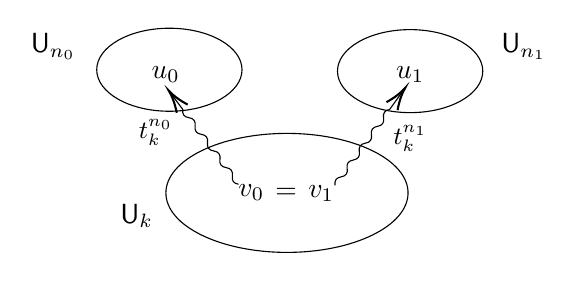
\begin{tikzpicture}[x=0.75pt,y=0.75pt,yscale=-1,xscale=1]
%uncomment if require: \path (0,300); %set diagram left start at 0, and has height of 300

%Shape: Ellipse [id:dp4815941303797192] 
\draw   (103.67,84.33) .. controls (103.67,73.29) and (119.34,64.33) .. (138.67,64.33) .. controls (158,64.33) and (173.67,73.29) .. (173.67,84.33) .. controls (173.67,95.38) and (158,104.33) .. (138.67,104.33) .. controls (119.34,104.33) and (103.67,95.38) .. (103.67,84.33) -- cycle ;
%Shape: Ellipse [id:dp17791572333330286] 
\draw   (219.67,85) .. controls (219.67,73.95) and (235.34,65) .. (254.67,65) .. controls (274,65) and (289.67,73.95) .. (289.67,85) .. controls (289.67,96.05) and (274,105) .. (254.67,105) .. controls (235.34,105) and (219.67,96.05) .. (219.67,85) -- cycle ;
%Shape: Ellipse [id:dp467313711776734] 
\draw   (137,143.67) .. controls (137,127.83) and (163.12,115) .. (195.33,115) .. controls (227.55,115) and (253.67,127.83) .. (253.67,143.67) .. controls (253.67,159.5) and (227.55,172.33) .. (195.33,172.33) .. controls (163.12,172.33) and (137,159.5) .. (137,143.67) -- cycle ;
%Straight Lines [id:da3638554959651593] 
\draw    (172,139.5) .. controls (169.67,139.16) and (168.67,137.82) .. (169.01,135.49) .. controls (169.35,133.16) and (168.35,131.82) .. (166.02,131.48) .. controls (163.69,131.14) and (162.69,129.8) .. (163.04,127.47) .. controls (163.38,125.14) and (162.38,123.8) .. (160.05,123.46) .. controls (157.72,123.13) and (156.72,121.79) .. (157.06,119.46) .. controls (157.4,117.13) and (156.4,115.79) .. (154.07,115.45) .. controls (151.74,115.11) and (150.74,113.77) .. (151.08,111.44) .. controls (151.42,109.11) and (150.42,107.77) .. (148.09,107.43) .. controls (145.76,107.09) and (144.76,105.75) .. (145.11,103.42) -- (144.31,102.35) -- (139.53,95.94) ;
\draw [shift={(138.33,94.33)}, rotate = 53.3] [color={rgb, 255:red, 0; green, 0; blue, 0 }  ][line width=0.75]    (10.93,-3.29) .. controls (6.95,-1.4) and (3.31,-0.3) .. (0,0) .. controls (3.31,0.3) and (6.95,1.4) .. (10.93,3.29)   ;
%Straight Lines [id:da2882231844046552] 
\draw    (218.5,140) .. controls (218.12,137.67) and (219.09,136.32) .. (221.42,135.94) .. controls (223.75,135.56) and (224.72,134.21) .. (224.34,131.88) .. controls (223.96,129.55) and (224.93,128.2) .. (227.26,127.83) .. controls (229.59,127.45) and (230.56,126.1) .. (230.18,123.77) .. controls (229.81,121.44) and (230.78,120.09) .. (233.11,119.71) .. controls (235.44,119.33) and (236.41,117.98) .. (236.03,115.65) .. controls (235.65,113.32) and (236.62,111.97) .. (238.95,111.59) .. controls (241.28,111.22) and (242.25,109.87) .. (241.87,107.54) .. controls (241.49,105.21) and (242.46,103.86) .. (244.79,103.48) -- (246.49,101.12) -- (251.16,94.62) ;
\draw [shift={(252.33,93)}, rotate = 125.75] [color={rgb, 255:red, 0; green, 0; blue, 0 }  ][line width=0.75]    (10.93,-3.29) .. controls (6.95,-1.4) and (3.31,-0.3) .. (0,0) .. controls (3.31,0.3) and (6.95,1.4) .. (10.93,3.29)   ;

% Text Node
\draw (128.83,81.4) node [anchor=north west][inner sep=0.75pt]  [font=\normalsize]  {$u_{0}$};
% Text Node
\draw (70.67,65.73) node [anchor=north west][inner sep=0.75pt]  [font=\normalsize]  {$\U_{n_{0}}$};
% Text Node
\draw (246.67,81.57) node [anchor=north west][inner sep=0.75pt]  [font=\normalsize]  {$u_{1}$};
% Text Node
\draw (297.33,65.73) node [anchor=north west][inner sep=0.75pt]  [font=\normalsize]  {$\U_{n_{1}}$};
% Text Node
\draw (170.67,138.23) node [anchor=north west][inner sep=0.75pt]  [font=\normalsize]  {$v_{0}$};
% Text Node
\draw (204.33,138.73) node [anchor=north west][inner sep=0.75pt]  [font=\normalsize]  {$v_{1}$};
% Text Node
\draw (113.83,147.73) node [anchor=north west][inner sep=0.75pt]  [font=\normalsize]  {$\U_{k}$};
% Text Node
\draw (122.67,107.07) node [anchor=north west][inner sep=0.75pt]  [font=\small]  {$t_{k}^{n_{0}}$};
% Text Node
\draw (245.33,109.73) node [anchor=north west][inner sep=0.75pt]  [font=\small]  {$t_{k}^{n_{1}}$};
% Text Node
\draw (188.5,140.4) node [anchor=north west][inner sep=0.75pt]  [font=\normalsize]  {$=$};


\end{tikzpicture}


}%

\label{fig:my_label}
\end{figure}

Even with this generalised lemma, we would get stuck in the proof for the case of the decoding. Indeed, if we have a code $a: \U_n$ type $A$ 
which erasure is $|A| = |a|$, then we cannot deduce much on $A$ itself as it could well be any type.
Nevertheless, we still know that $\Gamma \vdash A : \U_n$ holds in Russell-style because it is the same syntactic term as $a$. This should indicate that $A$ is a small type, i.e. a decoded type, and
in this setting we will prove that : \[\Gamma \vdash A = T_n(a)\]

Thus, we shall prove the following lemma, which is the most technical result of this paper. One of 
the reason for this, is that we want to keep the proof elementary, by relying only on basic syntactic arguments. We could also
have used stronger arguments such as normalisation, but this would make the proof less modular and algorithmic.
Still, we sketch such a proof at the end of the section.

\begin{lemma}[\formline{Equivalence.v}{813}{eraseinjty}] \label{mainuniverse}
    In $\mathcal{T}_T$, we have:
    \begin{enumerate}
    \item If $\Gamma \vdash A\; \type$ and $\Gamma \vdash B\; \type$ with $|A| = |B|$, then  $\Gamma \vdash A = B$.

    \item If $\Gamma \vdash t : \U_n$ and $\Gamma \vdash A \; \type$ with $|A| = |t|$, then $\Gamma \vdash A = T_n(a)$. 

    \item If $\Gamma \vdash u_0 : A_0$ and $\Gamma \vdash u_1 : A_1$ with $|u_0| = |u_1|$, then we have two cases:
    \begin{itemize}
        \item Either $\Gamma \vdash A_0 = A_1$ and $\Gamma \vdash u_0 = u_1 : A_0$.
        \item Or they are codes, such that $\Gamma \vdash A_0 = \U_{n_0}$, $\Gamma \vdash A_1 = \U_{n_1}$, and 
            there exists two convertible terms $\Gamma \vdash v_0 = v_1 : \U_k$ in a lower universe, which
            lifts to $u_0$ and $u_1$:

            \vspace{0.5em}

            \noindent
            \begin{minipage}{0.5\linewidth}
                \centering
                $\Gamma \vdash u_0 = t_k^{n_0}(v_0) : A_0$
            \end{minipage}
            \hfill
            \begin{minipage}{0.5\linewidth}
                \centering
                $\Gamma \vdash u_1 = t_k^{n_1}(v_1) : A_1$
        \end{minipage}
    \end{itemize}
    \end{enumerate}
\end{lemma}

\begin{proof}
    We prove the property by mutual induction on $A$ and $u_0$, proving the three statements at the same time. For each of the cases of
    the induction, we need a "catch-up" lemma which inverts the erasure hypothesis. Concretely the issue is that we cannot 
    deduce from $|u_1| = \Pi(A,B)$ that $u_1$ is a dependent product, as it could well be the decoding of a code $T_n(\Pi^n \; a \; b)$, or
    even a decoding of a lift $T_n(t_m^n(a))$. To solve this, we need to do another induction on $u_1$ for each case.

    We now present some of the key cases of the proof.\\

    \textit{Lambda abstraction.} If $u_0 = \lambda(C_0,B_0,b_0)$, then we necessarily have $A_0 = \Pi(C_0,B_0)$,
        and by inversion, the derivation $\Gamma \vdash u_0 : A_0$ looks like :

    \begin{mathparsmall}
      \ebrule{
        \hypo{\Gamma.C_0 \vdash b_0 : B_0}
        \infer1{\Gamma \vdash \lambda(C_0,B_0,b_0) : \Pi(C_0,B_0)}
      }
    \end{mathparsmall}

    Then $|u_0| = \lambda(|C_0|, |B_0|, |b_0|) = |u_1|$ and so $u_1$ is necessarily
    an abstraction or a lift. Now let's prove the property by induction on $u_1$.

    \begin{itemize}
        \item \underline{First case:} $u_1 = \lambda(C_1, B_1, b_1)$ with $|C_1| = |C_0|$, $|B_1| = |B_0|$, $|b_1| = |b_0|$.
    Also, by inversion $\Gamma \vdash u_1 : A_1$ is necessarily of the same shape. 
    Using the induction hypothesis on $C_0$ with $C_1$, we get $\Gamma \vdash C_0 = C_1$.
    Then, by lemma \ref{Transform} we get a derivation
    $\Gamma,C_0 \vdash b_1 : B_1$. Now we can apply the induction hypothesis on $b_0$ with $b_1$, and get two cases. 
    
    In the first case, we get directly derivations $\Gamma \vdash b_1 = b_0 : B_0$ and $\Gamma \vdash B_0 = B_1$,
    and using congruence equations we obtain the desired $\Gamma \vdash u_0 = u_1 : A_0$.
    
    In the second case, we get $\Gamma \vdash A_0 = \U_{n_0}$, from which we deduce $\Gamma \vdash \Pi(C_0,B_0) = \U_{n_0}$,
    which is a contradiction by lemma \ref{no-confusion}.

    \item \underline{Second case:} $u_1 = t_n^m(a)$, and we will show that this case is not possible.
        Indeed, we thus have $A_1 = \U_m$ and $|u_1| = |a| = |u_0|$ and we can apply the induction hypothesis
        on $a$, and in each case we obtain either $\Gamma \vdash A_0 = \U_m$ or $\Gamma \vdash A_0 = \U_{n_0}$, which
        are absurd because of lemma \ref{no-confusion}.
    \end{itemize}

    The case of lambda abstraction illustrated the main arguments used, and how no-confusion plays an 
    essential role to our arguments. However, in more complicated cases, we cannot always eliminate lifting
    cases.\\

    \textit{Code for a universe.} If $u_0$ is a code for a universe, then by inversion :
    \begin{mathparsmall}
      \ebrule{
        \hypo{}
        \infer1{\Gamma \vdash \U_m^{n_0} : \U_{n_0}}
      }
    \end{mathparsmall}
    Then $|u_0| = \U_m = |u_1|$ so we have two cases either $u_1 = \U_m^{n_1}$ or $u_1 = t_l^{n_1} (\U_m^l)$.

    \begin{itemize}
        \item \underline{First case :} We have $u_1 = \U_m^{n_1}$, and by inversion
    the following derivations : $\Gamma \vdash A_0 = \U_{n_0}$ and $\Gamma \vdash A_1 = \U_{n_1}$.
    If we define $k := \min{n_0,n_1}$ then we can construct derivations
    $\Gamma \vdash u_0 = t_k^{n_0} (\U_m^k)$ and $\Gamma \vdash u_1 = t_k^{n_1} (\U_m^k)$, with $\Gamma \vdash \U_m^k = \U_m^k : \U_k$.

    \item \underline{Second case :} We have $u_1 = t_l^{n_1} (\U_m^l)$, and by inversion the following
    derivations : $\Gamma \vdash A_0 = \U_{n_0}$ and $\Gamma \vdash A_1 = \U_{n_1}$. If we define $k := \min(l,n_0)$, we can construct derivations
    $\Gamma \vdash u_0 = t_k^{n_0} (\U_m^k)$ and $\Gamma \vdash u_1 = t_k^{n_1} (\U_m^k)$, with  $\Gamma \vdash \U_m^k = \U_m^k : \U_k$.
    \end{itemize}
\end{proof}



\begin{lemma}[\formline{Equivalence.v}{11}{simplifyinduction}]\label{Utile}
     Let's assume that : $\Gamma \vdash A_0 = \U_{n_0}$, $\Gamma \vdash A_1 = \U_{n_1}$ and 
     $\Gamma \vdash u_0 = t_k^{n_0}(v_0) : A_0$, $\Gamma \vdash u_1 = t_k^{n_1}(v_1) : A_1$ with
     $\Gamma \vdash v_0 = v_1 : \U_k$.

     Then if we additionally have  $\Gamma \vdash A_0 = A_1$, we get : $\Gamma \vdash u_0 = u_1: A_0$.
\end{lemma}
\begin{proof}
    By transitivity, we get $\Gamma \vdash \U_{n_0} = \U_{n_1}$ from which we can deduce $n_0 = n_1$ using
    injectivity of universes. Hence, $u_0$ and $u_1$ are codes living in the same universe.
    Via congruence, we get $\Gamma \vdash t_k^{n_0}(v_0) = t_k^{n_0}(v_1)$,
    from which we deduce $\Gamma \vdash u_0 = u_1 : A_0$ by transitivity.
\end{proof}


Hence, we deduce the following corollary, which states that if we have two judgments
in $\mathcal{T}_T$ which are syntactically equal in $\mathcal{T}_R$ (when removing coercions, lifts...), then
they are provably convertible in $\mathcal{T}_T$. This already means that the Tarski system is not much stronger than
the Russell one, in the sense that if two term differ only by their explicit coercion, then they have the same
computational behaviour.

\begin{corollary}[\formline{Equivalence.v}{1128}{eraseinjtermplus} Judgemental injectivity of erasure]\label{uniqueness}
    If $\Gamma \vdash u_0 : A_0$ and $\Gamma \vdash u_1 : A_1$ in $\mathcal{T}_T$ and $|u_0| = |u_1|$,
    with the additional hypothesis $|A_0| = |A_1|$, then : $\Gamma \vdash A_0 = A_1$ and 
    $\Gamma \vdash u_0 = u_1 : A_0$.
\end{corollary}

\begin{proof}
    We apply lemma \ref{mainuniverse} on the equality $|A_0| = |A_1|$ to get $\Gamma \vdash A_0 = A_1$, and on
    $|u_0| = |u_1|$ to get the two cases. In the first one, we directly have $\Gamma \vdash u_0 = u_1 : A_0$,
    and in the second one, we use lemma \ref{Utile} to get the derivation.
\end{proof}

Now we prove the following theorem, stating the formal equivalence between the two systems:

\begin{theorem}[\formline{Equivalence.v}{1379}{sectionctx} Section of erasure]\label{equT1T2}
    If $\Gamma \vdash J$ in the system $\mathcal{T}_R$, then there exists a unique, up to conversion judgment
    $\Gamma_1 \vdash J_1$ in the system $\mathcal{T}_T$ such that $|\Gamma_1| = \Gamma$ and $|J_1| = J$.
\end{theorem}

\begin{proof}
    Uniqueness up to conversion follows directly from the previous lemma. We have to construct the derivation 
    by induction on the rules of $\mathcal{T}_R$, making an extensive use of the previous lemma for rules with two premises. Indeed,
    when using the induction hypothesis on two premises, we need to make sure that the same types have 
    the same translations. To illustrate this, we detail the case of the product.\\

    \textit{Dependent Product.} If the last rule applied in $\mathcal{T}_R$ is :
    \begin{mathparsmall}
      \ebrule{
        \hypo{\Pi_1}
        \infer1{\Gamma \vdash A \; \type}
        \hypo{\Pi_2}
        \infer1{\Gamma.A \vdash B \; \type}
        \infer2{\Gamma \vdash \Pi(A,B) \; \type}
      }
    \end{mathparsmall}

        Then, by the induction hypothesis we get derivations 
        $\Gamma' \vdash A' \; \type$ and $\Gamma'',A'' \vdash B' \; \type$ in $\mathcal{T}_T$ such that 
         $|\Gamma'| = |\Gamma''| = \Gamma$ and $|A''| = |A'| = A$. By lemma \ref{uniqueness}, we get $\Gamma \vdash A = A'$, and  the contexts
        $\Gamma'$ and $\Gamma''$ are convertible. We can thus transform the second derivation to get $\Gamma',A' \vdash B' \; \type$.
        Therefore, we can construct the derivation for $\Gamma \vdash \Pi(A',B') \; \type$ in $\mathcal{T}_T$.
\end{proof}

This finally proves that any judgement in Russell-Style can be lifted uniquely to a judgement in Tarski-Style, proving
the equivalence between $\mathcal{T}_T$ and $\mathcal{T}_R$ by exhibiting a section of the forgetful map.

\begin{remark}
To prove this equivalence result, we could have relied on normalisation to simplify the proofs, at
the cost of relying on less elementary properties of the theory. In fact, if we proved normalisation for
$\mathcal{T}_R$ as well, we could construct the derivation of \ref{equT1T2} by an induction on normal forms.
Then, by showing that the erasure map $|.|$ commutes with $\nf(.)$, we would obtain the equivalence result.
However, we chose to not rely on such results as they are stronger and not needed.
\end{remark}

\section{Unannotated syntax ($\mathcal{T}_R$ and $\mathcal{T}_P$)}\label{sectionT2T2'}

Finally, we prove our last equivalence result between $\mathcal{T}_R$ and $\mathcal{T}_P$, relating
annotated and unannotated syntax. Concretely, the target theory $\mathcal{T}_P$ is the closest we can
get to a presentation as a Pure Type System of Martin-Löf's type theory with a cumulative hierarchy of universes.
This section is a direct adaptation of the arguments of \citet{Streicher} to our setting. Notably, we need
to adapt the arguments because the theory $\mathcal{T}_R$ does not enjoy uniqueness of types, precisely because
of cumulativity.

Just as we did for the previous equivalence result, we prove that the forgetful map $\strip$ preserves
derivations.

\begin{theorem}
    If $\Gamma \vdash J$ in $\mathcal{T}_R$, then we have a derivation $\strip(\Gamma) \vdash \strip(J)$ in $\mathcal{T}_P$.
\end{theorem}
\begin{proof}
    We just need to prove that the stripping of rules in $\mathcal{T}_R$ are admissible in $\mathcal{T}_P$, which
    is quite easy as each rule in $\mathcal{T}_R$ corresponds directly to a rule of $\mathcal{T}_P$. Then, the theorem
    is proved by an induction on the derivation which replaces rules in $\mathcal{T}_R$ by the admissible ones in $\mathcal{T}_P$.
\end{proof}

Now, following the ideas of \citet{Streicher}, we want to prove that two terms or types which
become syntactically equal after erasing the annotations with $\strip$ are convertible in $\mathcal{T}_R$. Here, 
types are not unique because of cumulativity, so we could well have $\strip(u_0) = \strip(u_1)$ without
necessarily having $u_0$ and $u_1$ convertible. This is due to the codomain annotations of $\lambda$-abstractions, which are erased by $\strip$ and are subject to cumulativity, as shown by the following counter-example.

\begin{example}\label{ex:cumul-lam}
    For $n < p$, the terms $f_0 = \lambda(\U_n,\U_n,v_0) : \Pi(\U_n,\U_n)$ and $f_1 = \lambda(\U_n,\U_p,v_0) : \Pi(\U_n,\U_p)$ have the same stripping $\lambda(\U_n,v_0)$,
    but neither their types $\Pi(\U_n,\U_n)$ and $\Pi(\U_n,\U_p)$ nor $f_0$ and $f_1$ are convertible.
    Yet, when applied to $\U_0$ (for $0 < n < p$), the applications $u_0 = \app(\U_n,\U_n,f_0,\U_0)$ and $u_1 = \app(\U_n,\U_p,f_1,\U_0)$ both have type $\U_p$ by cumulativity, have the same stripping $(\lambda(\U_n,v_0))\;\U_0$, and are convertible: $\Gamma \vdash u_0 = u_1 : \U_p$.
\end{example}

As Example \ref{ex:cumul-lam} illustrates, even if two applications $u_0$ and $u_1$ are compared at a common type, the functions $f_0$ and $f_1$ being applied may have types $\Pi(\U_n,\U_n)$ and $\Pi(\U_n,\U_p)$ that differ by cumulativity \emph{under $\Pi$}.
Although $\mathcal{T}_R$ has no primitive sub-typing judgement for $\Pi$-types, we can relate such terms by defining explicit coercions into a common upper type (a \emph{join}) using $\eta$-expansion, with cumulativity acting at the leaves.

\begin{definition}[Joins and coercions]\label{def:join}
    We inductively define the judgement $\Gamma \vdash \JoinTy(T_0, T_1, L) \leadsto (\coe_0, \coe_1)$, relating types $T_0, T_1$ to a common join $L$ via coercion operations $\coe_0, \coe_1$, by the following inference rules:
    \begin{mathparsmall}
      \ebrule{
        \hypo{\Gamma \vdash T_0 = L}
        \hypo{\Gamma \vdash T_1 = L}
        \infer2{\Gamma \vdash \JoinTy(T_0, T_1, L) \leadsto (\Id, \Id)}
      }
      \and
      \ebrule{
        \hypo{\Gamma \vdash T_0 = \U_k}
        \hypo{\Gamma \vdash T_1 = \U_m}
        \infer2{\Gamma \vdash \JoinTy(T_0, T_1, \U_{\max(k,m)}) \leadsto (\Id, \Id)}
      }
      \and
      \ebrule{
        \hypo{\Gamma \vdash T_0 = \Pi(A, B_0)}
        \hypo{\Gamma \vdash T_1 = \Pi(A, B_1)}
        \hypo{\Gamma.A \vdash \JoinTy(B_0, B_1, L') \leadsto (\coe_0, \coe_1)}
        \infer3{\Gamma \vdash \JoinTy(T_0, T_1, \Pi(A, L')) \leadsto (\pi_{A,B_0,L'}(\coe_0), \pi_{A,B_1,L'}(\coe_1))}
      }
    \end{mathparsmall}
    where the action of a coercion on a term $t$ is defined inductively by:
    \begin{align*}
        \Id(t) &:= t,\\
        \pi_{A,B,L'}(\coe)(t) &:= \lambda(A, L', \coe(\app(A\p, B\p^+, t\p, v_0))).
    \end{align*}
\end{definition}

By induction on the join derivation, joins are symmetric, transport along type conversions $\Gamma \vdash T'_i = T_i$, and are stable under substitution $\sigma : \Delta \to \Gamma$, with $(\coe_i(t))\sigma = \coe_{i\sigma}(t\sigma)$. Coercions are well-typed ($\Gamma \vdash t : T_i \implies \Gamma \vdash \coe_i(t) : L$), congruent, and compute under application by the $\beta$-rule:
\[\Gamma \vdash \app(A, L', \pi_{A,B_i,L'}(\coe_i)(t), a) = \coe_{i[a]}(\app(A, B_i, t, a)) : L'[a].\]

When $T_0$ and $T_1$ are convertible, coercions into their join are injective up to conversion (analogously to Lemma \ref{Utile}).

\begin{lemma}[Diagonal lemma]\label{lem:join-diag}
    If $\Gamma \vdash \JoinTy(T_0, T_1, L) \leadsto (\coe_0, \coe_1)$, $\Gamma \vdash t_0 : T_0$, $\Gamma \vdash t_1 : T_1$, and $\Gamma \vdash \coe_0(t_0) = \coe_1(t_1) : L$, then $\Gamma \vdash T_0 = T_1$ implies $\Gamma \vdash t_0 = t_1 : T_0$.
\end{lemma}
\begin{proof}
    By induction on $\Gamma \vdash \JoinTy(T_0, T_1, L) \leadsto (\coe_0, \coe_1)$. The conversion case is immediate.\\

    \textit{Universe case.} $\Gamma \vdash \U_k = \U_m$ gives $k = m$ by universe injectivity, so $L = \U_{\max(k,k)} = \U_k$.\\

    \textit{Product case.} $\Gamma \vdash \Pi(A, B_0) = \Pi(A, B_1)$ gives $\Gamma.A \vdash B_0 = B_1$ by $\Pi$-injectivity. Weakening $\Gamma \vdash \pi_{A,B_0,L'}(\coe_0)(t_0) = \pi_{A,B_1,L'}(\coe_1)(t_1) : \Pi(A, L')$ to $\Gamma.A$, applying both sides to $v_0$, and using the $\beta$-rule yields $\Gamma.A \vdash \coe_0(h_0) = \coe_1(h_1) : L'$ where $h_i = \app(A\p, B_i\p^+, t_i\p, v_0)$. The induction hypothesis gives $\Gamma.A \vdash h_0 = h_1 : B_0$, and congruence of $\lambda$ together with the $\eta$-rule concludes $\Gamma \vdash t_0 = t_1 : T_0$.
\end{proof}

We now state and prove the main lemma of this section by structural induction on the syntax, comparing terms at the join of their types.

\begin{lemma}\label{streichT2T2'}
    In $\mathcal{T}_R$, we have:
    \begin{enumerate}
        \item If $\Gamma \vdash u_0 : T_0$ and $\Gamma \vdash u_1 : T_1$ with $\strip(u_0) = \strip(u_1)$, then there exists a join $\Gamma \vdash \JoinTy(T_0, T_1, L) \leadsto (\coe_0, \coe_1)$ such that $\Gamma \vdash \coe_0(u_0) = \coe_1(u_1) : L$.
        \item If $\Gamma \vdash A_0 \; \type$ and $\Gamma \vdash A_1 \; \type$ with $\strip(A_0) = \strip(A_1)$, then $\Gamma \vdash A_0 = A_1$.
    \end{enumerate}
\end{lemma}

\begin{proof}
    By mutual structural induction on $u_0$ and $A_0$. Statement (2) follows directly from statement (1), since for $\Gamma \vdash A_i : \U_{l_i}$, any join of $\U_{l_0}$ and $\U_{l_1}$ gives $\Gamma \vdash A_0 = A_1 : \U_{\max(l_0, l_1)}$ by no-confusion and universe injectivity.
    For statement (1), inversion on $\Gamma \vdash u_i : T_i$ gives the principal type $P_i$ of $u_i$, which is related to $T_i$ either by conversion or by universe cumulativity $\U_k \leq \U_m$. It therefore suffices to construct a join for the principal types $P_0, P_1$.

    Since $\strip(u_0) = \strip(u_1)$, $u_0$ and $u_1$ have the same head constructor. Variables, universes, and products are straightforward. For $\lambda$-abstractions $u_i = \lambda(A_i, B_i, b_i)$, statement (2) gives $\Gamma \vdash A_0 = A_1$. After transporting $b_1 : B_1$ to context $\Gamma.A_0$, the induction hypothesis on $b_0, b_1$ yields a join $\Gamma.A_0 \vdash \JoinTy(B_0, B_1, L') \leadsto (\coe_0, \coe_1)$ with $\Gamma.A_0 \vdash \coe_0(b_0) = \coe_1(b_1) : L'$, which lifts to a product join on $\Pi(A_0, L')$ via the $\beta$-rule under $\lambda$. We detail the remaining case of function application.\\

    \textit{Function application.} If $u_0 = \app(C_0, D_0, c_0, a_0)$, then $u_1 = \app(C_1, D_1, c_1, a_1)$ with $\strip(c_0) = \strip(c_1)$ and $\strip(a_0) = \strip(a_1)$. By inversion, $\Gamma \vdash c_i : \Pi(C_i, D_i)$ and $\Gamma \vdash a_i : C_i$, with principal type $P_i = D_i[a_i]$.
    By the induction hypothesis, we have a join $\Gamma \vdash \JoinTy(\Pi(C_0, D_0), \Pi(C_1, D_1), L) \leadsto (\coe_0, \coe_1)$ with $\Gamma \vdash \coe_0(c_0) = \coe_1(c_1) : L$, and a join for $a_0, a_1$ on $C_0, C_1$. By no-confusion, the join for $c_0, c_1$ is either a conversion join or a product join:
    \begin{itemize}
        \item \underline{Conversion join:} We have $\Gamma \vdash \Pi(C_0, D_0) = \Pi(C_1, D_1)$ and $\Gamma \vdash c_0 = c_1 : \Pi(C_0, D_0)$. By $\Pi$-injectivity, $\Gamma \vdash C_0 = C_1$ and $\Gamma.C_0 \vdash D_0 = D_1$. Lemma \ref{lem:join-diag} on the join for $a_0, a_1$ gives $\Gamma \vdash a_0 = a_1 : C_0$, and congruence of $\app$ concludes.
        \item \underline{Product join:} We have $L = \Pi(A, L')$ with $\Gamma \vdash \Pi(C_i, D_i) = \Pi(A, B_i)$ and $\Gamma.A \vdash \JoinTy(B_0, B_1, L') \leadsto (\coe_{B_0}, \coe_{B_1})$. By $\Pi$-injectivity, $\Gamma \vdash C_i = A$ and $\Gamma.C_i \vdash D_i = B_i$. In particular, $\Gamma \vdash C_0 = C_1$, so Lemma \ref{lem:join-diag} again gives $\Gamma \vdash a_0 = a_1 : A$. Applying $\Gamma \vdash \coe_0(c_0) = \coe_1(c_1) : \Pi(A, L')$ to $a_0$, using the $\beta$-computation rule for coercions on both sides, and congruence of $\app$ yields:
        \[\Gamma \vdash \coe_{B_0[a_0]}(u_0) = \coe_{B_1[a_0]}(u_1) : L'[a_0],\]
        which is a join for $B_0[a_0]$ and $B_1[a_0]$, and hence for $D_0[a_0]$ and $D_1[a_1]$.
    \end{itemize}
\end{proof}

Combining Lemma \ref{streichT2T2'} with the diagonal lemma (Lemma \ref{lem:join-diag}), we deduce the following direct corollary, analogous to Corollary \ref{uniqueness} of the previous section.

\begin{corollary}\label{cor:strip-uniq}
    If $\Gamma \vdash u_0 : A_0$ and $\Gamma \vdash u_1 : A_1$ in $\mathcal{T}_R$ with $\strip(u_0) = \strip(u_1)$ and $\strip(A_0) = \strip(A_1)$, then $\Gamma \vdash A_0 = A_1$ and $\Gamma \vdash u_0 = u_1 : A_0$.
\end{corollary}
\begin{proof}
    If $\strip(A_0) = \strip(A_1)$, Lemma \ref{streichT2T2'}.(2) gives $\Gamma \vdash A_0 = A_1$. Then Lemma \ref{streichT2T2'}.(1) and Lemma \ref{lem:join-diag} yield $\Gamma \vdash u_0 = u_1 : A_0$.
\end{proof}

Finally, we can show the following theorem, which exhibits the section of the forgetful map $\strip$, showing the equivalence
of $\mathcal{T}_R$ and $\mathcal{T}_P$.

\begin{theorem}\label{equT2T2'}
    If $\Gamma \vdash J$ in $\mathcal{T}_P$, then we have a unique up to conversion judgment 
    $\Gamma' \vdash J'$ in $\mathcal{T}_R$ such that $\strip(\Gamma') = \Gamma$ and $\strip(J') = J$.
\end{theorem}
\begin{proof}
    By induction on the derivation $\Gamma \vdash J$, using Corollary \ref{cor:strip-uniq}, we construct a derivation in $\mathcal{T}_R$.
    The main point is that the typing annotations can be inferred from the derivation, and that Corollary \ref{cor:strip-uniq} gives
    us uniqueness up to conversion for rules with shared terms or types in their premises. 
\end{proof}

In $\mathcal{T}_P$, we could also remove the judgement $\Gamma \vdash A\; \type$ to manipulate only universes,
in a completely Russellian style. In such a system, there is no top-level of types and a type is simply a term
of a certain universe.
We can also consider named variables instead of de Bruijn indices, to get a theory presented exactly like a pure type
system, with the additional rule for cumulativity.

If we wanted to go even further, we could also remove the annotation of the variable from the lambda abstraction, again
following \citet{Streicher}. However to do so, we crucially need to rely on the full normalisation result,
as removing this annotation can lead to multiple non-convertible derivations for the same judgement, as shown by the following example.
    
\begin{example}
        We have two derivations : $t :\U_n \vdash \lambda \,x.x : \Pi(\U_n,\U_n)$ and $t :\U_n \vdash \lambda \,x.x : \Pi(\U_n,\U_p)$, which are not convertible when $n<p$.
        Then we can construct the same derivation from those two premises: \[t :\U_n \vdash (\lambda \,y.t) \; (\lambda \,x.x) : \U_n\]
\end{example}

\section{Extensions of our result}

In this section, we illustrate the modularity of our proof method by showing that it extends to more complicated systems.
In fact, we believe that the proof should extend to various flavours of type theories, as long as they satisfy definitional inversion.

For instance, we describe how to extend our equivalence result to the theory of \citet{polymorphism, bcde2026}, with explicit universe polymorphism and cumulative universes indexed by internal levels.
For the theory without constraints, the proof of the previous sections can be adapted directly by simply making the reasoning on levels internal to the theory.
However, for a theory with constraints, things get more complicated. 

In this system, contexts can be extended with level variables $\Gamma, \alpha$ and level constraints $\Gamma, \psi$, we also have level and constraint products $[\alpha]A$, $[\psi]A$, along with a collapse element $\emptyset$ in inconsistent level contexts.

First, to relate the Tarski and Russell presentations ($\mathcal{T}_T$ and $\mathcal{T}_R$). When we look closely at what was needed in Section \ref{sectionT1T2}, we observe that for universe levels we only need to take suprema and infima. In fact, the lower universe $\U_k$ of Lemma \ref{mainuniverse} is given by $\min(n_0,n_1)$ in the base cases. To reconstruct this operation internally, we observe that in any consistent context, if a constraint $l \leq n_0$ and $l \leq n_1$ holds, we can use the decidability of the arithmetic on levels.

Second, to relate the annotated and unannotated Russell presentations ($\mathcal{T}_R$ and $\mathcal{T}_P)$, where $\strip$ also erases the type annotations on $\langle \alpha \rangle_A u$, $\langle \psi \rangle_A t$, and $t_A l$), we extend the join and coercion method of Section \ref{sectionT2T2'}. Because cumulativity does not act structurally on $[\alpha]A$ or $[\psi]A$, we extend Definition \ref{def:join} with join rules for $[\alpha]B_i$ and $[\psi]B_i$, where universe joins use the internal supremum $\U_{k \vee m}$ and the corresponding coercions are defined by $\eta$-expansion.

\[
    \coe_{[\alpha]B \leq [\alpha]L'}(t) := \langle \alpha \rangle_{L'}\,\coe_{B \leq L'}((t\p)_{B\p^+}\,\alpha), \qquad
    \coe_{[\psi]B \leq [\psi]L'}(t) := \langle \psi \rangle_{L'}\,\coe_{B \leq L'}(t).
\]
For the diagonal lemma (Lemma \ref{lem:join-diag}) to go through for constraint products, we add the natural $\eta$-rule for constraint products :
\[\Gamma \vdash \langle \psi \rangle_A t  = t : [\psi]A \quad \text{when} \quad \Gamma \vdash t : [\psi]A\]
Moreover, since $[\psi]A = A$ holds whenever $\psi$ is valid in $\Gamma$, a constraint product is not necessarily distinct from a universe, $\Pi$-type, or level product. Thus, the domain model should have a guard-aware no-confusion property stating that in a consistent context, if $[\psi]A$ is convertible to $\U_l$, $\Pi(C,B)$, or $[\alpha]B$, then $\psi$ is valid in $\Gamma$.


\section{Conclusion and Future Work}

We proved that the Generalised Algebraic Theory and Pure Type System
presentations of Martin Löf's Type Theory are equivalent. More specifically, we related 
\textit{Tarski} and \textit{Russell} presentations of cumulative universe hierarchies. We also extended
our equivalence result to theories with data types or universe polymorphism.

Those equivalence results are fundamental to justify the common, but informal, practice of using implicit syntax
and Russell universes for practitioners of type theory. Notably, our result rigorously legitimates the interpretation of
implicit presentations in the usual models of type theory, which usually applies to annotated syntax. Our
result also shows that Russellian systems can be used as well to present this initial models of type theory, thus
extending initiality results to more realistic syntaxes.

Our proof relies on definitional inversion, which we prove using the domain-theoretic approach of \citet{definitional-inv}. 
Crucially, we do not rely on normalisation and our proof is completely elementary.
We believe that our proof technique can be adapted to a variety of extensions and more sophisticated type theories.\\

\textbf{\textit{Future work.}} In this paper, we did not consider cumulativity with a structural sub-typing relation for the sake of simplicity, and could lead to issues with general inductive types as pointed out by \citet{Luo}.

In fact, structural subtyping on inductive types such as a the type of lists $\lst(.)$ breaks
canonicity: we can coerce $\mathsf{nil}_{\U_0} : \lst(\U_1)$, but we do not have $\mathsf{nil}_{\U_0} = \mathsf{nil}_{\U_1}$,
unless we manually add the equation.

Yet, structural sub-typing would provide a more convenient manipulation of universes in a practical proof
assistant. The issues mentioned for sub-typing of the introduction can be seen as a kind of anomaly of the syntax, and 
as a lack of proper equations. The recent work of \citet{AdapTT} presents a general framework which would provide automatically the necessary
equations to solve this issue, and we hope that the results of this paper could be extended to this setting.\\

\textbf{\textit{Acknowledgement.}} We thank Meven Lennon-Bertrand for his useful feedback on the first drafts
of this work, and for his comments on the mechanized proof.

\bibliography{main}

\appendix
\section{Appendix : Type systems}\label{Rules}

\subsection{The system $\mathcal{T}_T$ : Tarski universes}

We specify the system $\mathcal{T}_T$ with derivation rules.
This formulation with rules will be useful to prove properties by induction.
We start with the typing judgments $a : A$ and the well-formed type judgment $A \;\type$ :

\begin{mathparsmall}
  \ebrule{
    \hypo{\Gamma \vdash A \;\type}
    \infer1{\Gamma.A \vdash v_0 : A\p}
  }
  \and
  \ebrule{
    \hypo{\Gamma \vdash v_n:A}
    \hypo{\Gamma \vdash B \;\type}
    \infer2{\Gamma.B \vdash v_{n+1} : A\p}
  }
  \and
  \ebrule{
    \hypo{\Gamma \vdash A \;\type}
    \hypo{\Gamma.A \vdash B \;\type}
    \infer2{\Gamma \vdash \Pi(A, B) \;\type}
  }
  \and
  \ebrule{
    \hypo{\Gamma.A \vdash b: B}
    \hypo{\Gamma.A \vdash B \;\type}
    \hypo{\Gamma \vdash A \;\type}
    \infer3{\Gamma \vdash \lambda(A,B,b) : \Pi (A, B)}
  }
  \and
  \ebrule{
    \hypo{\Gamma \vdash c:\Pi(A, B)}
    \hypo{\Gamma.A \vdash a: A}
    \hypo{\Gamma.A \vdash B \;\type}
    \hypo{\Gamma \vdash A \;\type}
    \infer4{\Gamma \vdash \app(A,B,c,a) : B[a]}
  }
  \and
  \ebrule{
    \hypo{}
    \infer1{\Gamma \vdash \U_n \;\type}
  }
  \and
  \ebrule{
    \hypo{\Gamma \vdash a: \U_n}
    \hypo{\Gamma.T_n(a) \vdash b: \U_n}
    \hypo{\Gamma \vdash T_n(a) \;\type}
    \infer3{\Gamma \vdash \Pi^n \; a \; b: \U_n}
  }
  \and
  \ebrule{
    \hypo{\Gamma \vdash a:\U_n}
    \infer1{\Gamma \vdash T_n(a) \;\type}
  }
  \and
  \ebrule{
    \hypo{}
    \infer1[($m<n$)]{\Gamma \vdash \U_m^n: \U_n}
  }
  \and
  \ebrule{
    \hypo{\Gamma \vdash a: \U_n}
    \infer1[($n\leq p$)]{\Gamma \vdash t_m^n(a): \U_p}
  }
  \and
  \ebrule{
    \hypo{\Gamma \vdash a: A}
    \hypo{\Gamma \vdash A = B}
    \infer2{\Gamma \vdash a:B}
  }
  \ebrule{
    \hypo{\Gamma \vdash a=a' : A}
    \hypo{\Gamma \vdash A = B}
    \infer2{\Gamma \vdash a=a':B}
  }
  \and
  \ebrule{
    \hypo{\Gamma \vdash A = B}
    \hypo{\Gamma \vdash A = C}
    \infer2{\Gamma \vdash B = C}
  }
  \and
  \ebrule{
    \hypo{A \;\type}
    \infer1{A=A}
  }
  \and
  \ebrule{
    \hypo{\Gamma \vdash a=b : A}
    \hypo{\Gamma \vdash a=c : A}
    \infer2{\Gamma \vdash b=c:A}
  }
  \and
  \ebrule{
    \hypo{a:A}
    \infer1{a=a:A}
  }
  \and
  \ebrule{
    \hypo{\Gamma \vdash A = A'}
    \hypo{\Gamma.A \vdash B = B'}
    \infer2{\Gamma \vdash \Pi(A, B) = \Pi(A', B')}
  }
  \and
  \ebrule{
    \hypo{\Gamma.A \vdash b: B}
    \hypo{\Gamma \vdash a:A}
    \infer2[($\beta$-rule)]{\Gamma \vdash \app(A,B,\lambda(A,B,b),a) = b[a] : B[a]}
  }
  \and
  \ebrule{
    \hypo{f: \Pi \; A \; B}
    \infer1[($\eta$-rule)]{f = \lambda(A,B,\app(A\p,B\p^+,f\p, v_0)) : \Pi(A, B)}
  }
  \and
  \ebrule{
    \hypo{\Gamma \vdash a = a': \U_n}
    \infer1{\Gamma \vdash T_n(a) = T_n(a')}
  }
  \and
  \ebrule{
    \hypo{\Gamma \vdash a = a': \U_n}
    \infer1[($n\leq p$)]{\Gamma \vdash t_n^p(a) = t_n^p(a'): \U_p}
  }
  \and
  \ebrule{
    \hypo{\Gamma \vdash a: \U_n}
    \hypo{\Gamma,T_n(a) \vdash b: \U_n}
    \infer2{T_n(\Pi^n \; a \; b) = \Pi(T_n(a),T_n(b))}
  }
  \and
  \ebrule{
    \hypo{\Gamma \vdash a: \U_n}
    \hypo{\Gamma,T_n(a) \vdash b: \U_n}
    \infer2[($n\leq p$)]{t_n^p(\Pi^n \; a \; b) = \Pi^p(t_n^p(a),t_n^p(b))}
  }
  \and
  \ebrule{
    \hypo{}
    \infer1{\Gamma \vdash T_n(\U_m^n) = \U_m}
  }
  \and
  \ebrule{
    \hypo{}
    \infer1[($n\leq p$)]{\Gamma \vdash t_n^p(\U_m^n) = \U_m^p : \U_p}
  }
  \and
  \ebrule{
    \hypo{\Gamma \vdash a : \U_m}
    \infer1[($m \leq n$)]{\Gamma \vdash T_n(t_m^n(a)) = T_m(a)}
  }
  \and
  \ebrule{
    \hypo{\Gamma \vdash a : \U_m}
    \infer1[($m\leq n\leq p$)]{\Gamma \vdash t_n^p(t_m^n(a)) = t_m^p(a): \U_p}
  }
\end{mathparsmall}

We also require the rules that makes $=$ a congruence, but we omit those rules for brevity.

\subsection{The system $\mathcal{T}_G$ : explicit substitutions}

The system $\mathcal{T}_G$ is really close to $\mathcal{T}_T$, the only difference is that substitiutions
are explicit : they appear directly in the syntax. Hence, the syntax is given by :
\begin{gather*}
    \Gamma,\Delta ::= () \; | \; \Gamma.A\\
    A,B ::=  \Pi \; A \; B \;|\; \U_n \; | \; T_n(a) \; | \; A \sigma\\
    a,b ::= \app(A,B,c,a) \; | \; \lambda(A,B,b) \; | \; t_m^n(a) \; | \; \U_m^n \; | \; \Pi^n \; a \; b \; | \; \q_\Gamma \; | \; a\sigma \\
    \sigma , \delta ::= \sigma \delta \; | \; \Id_\Gamma \; | \; \p_{\Gamma,\Gamma.A} \; | \; [a] \; | \; \sigma^{+(A)}
\end{gather*}
The rules are the same as $\mathcal{T}_T$, with only one modification for variables, that are replaced by the rule
for $\q$ :

\begin{mathparsmall}
  \ebrule{
    \hypo{\Gamma \vdash A \;\type}
    \infer1{\Gamma.A \vdash q_{\Gamma.A} : A\p_{\Gamma,\Gamma.A}}
  }
\end{mathparsmall}

Then, we have rules for substitutions :

\begin{mathparsmall}
  \ebrule{
    \hypo{\Gamma \vdash}
    \infer1{\vdash \Id_\Gamma : \Gamma \rightarrow \Gamma}
  }
  \and
  \ebrule{
    \hypo{\Gamma \vdash A \; \type}
    \infer1{\vdash \p_{\Gamma,\Gamma.A} : \Gamma.A \rightarrow \Gamma}
  }
  \and
  \ebrule{
    \hypo{\Gamma \vdash a:A}
    \infer1{\vdash [a] : \Gamma \rightarrow \Gamma.A}
  }
  \and
  \ebrule{
    \hypo{\vdash \sigma : \Delta \rightarrow \Gamma}
    \hypo{\Gamma \vdash A \; \type}
    \infer2{\vdash \sigma^{+(A)}  : \Delta.A\sigma \rightarrow \Gamma.A}
  }
  \and
  \ebrule{
    \hypo{\vdash \sigma : \Delta \rightarrow \Gamma}
    \hypo{\vdash \delta : \Theta \rightarrow \Delta}
    \infer2{\vdash \sigma \delta : \Theta \rightarrow \Gamma}
  }
  \and
  \ebrule{
    \hypo{\vdash \sigma : \Delta \rightarrow \Gamma}
    \hypo{\Gamma \vdash A \; \type}
    \infer2{\Delta \vdash A \sigma \; \type}
  }
  \and
  \ebrule{
    \hypo{\vdash \sigma : \Delta \rightarrow \Gamma}
    \hypo{\Gamma \vdash t : A}
    \infer2{\Delta \vdash t \sigma \; \type}
  }
  \ebrule{
    \hypo{\vdash \sigma : \Delta \rightarrow \Gamma}
    \infer1{\vdash \sigma \Id_\Delta = \sigma : \Delta \rightarrow \Gamma}
  }
  \and
  \ebrule{
    \hypo{\vdash \sigma : \Delta \rightarrow \Gamma}
    \infer1{\vdash \Id_\Gamma \sigma = \sigma : \Delta \rightarrow \Gamma}
  }
  \and
  \ebrule{
    \hypo{\Gamma \vdash a = a' : A}
    \infer1{\vdash [a] = [a'] : \Gamma \rightarrow \Gamma.A}
  }
  \and
  \ebrule{
    \hypo{\vdash \sigma : \Delta \rightarrow \Gamma}
    \hypo{\vdash \delta : \Theta \rightarrow \Delta}
    \hypo{\vdash \nu : \Xi \rightarrow \Theta}
    \infer3{\vdash (\sigma \delta)\nu = \sigma(\delta \nu) : \Xi \rightarrow \Gamma}
  }
  \and
  \ebrule{
    \hypo{\vdash \sigma = \delta : \Delta \rightarrow \Gamma}
    \hypo{\vdash \sigma = \nu : \Delta \rightarrow \Gamma}
    \infer2{\vdash \sigma = \nu : \Delta \rightarrow \Gamma}
  }
  \and
  \ebrule{
    \hypo{\vdash \sigma = \sigma' : \Delta \rightarrow \Gamma}
    \hypo{\vdash \delta : \Theta \rightarrow \Delta}
    \infer2{\vdash \sigma\delta = \sigma'\delta : \Theta \rightarrow \Gamma}
  }
  \and
  \ebrule{
    \hypo{\vdash \sigma = \sigma' : \Delta \rightarrow \Gamma}
    \hypo{\vdash \delta : \Gamma \rightarrow \Theta}
    \infer2{\vdash \delta\sigma = \delta\sigma' : \Delta \rightarrow \Theta}
  }
  \and
  \ebrule{
    \hypo{\Gamma \vdash \Pi(A,B) \; \type}
    \hypo{\vdash \sigma : \Delta \rightarrow \Gamma}
    \infer2{\Delta \vdash \Pi(A,B)\sigma = \Pi(A\sigma,B\sigma^{+(A)})}
  }
  \and
  \ebrule{
    \hypo{\Gamma \vdash \lambda(A,B,b) : \Pi(A,B)}
    \hypo{\vdash \sigma : \Delta \rightarrow \Gamma}
    \infer2{\Delta \vdash \lambda(A,B,b)\sigma = \lambda(A\sigma,B\sigma^{+(A)},b\sigma^{+(A)}) : \Pi(A\sigma,B\sigma^{+(A)})}
  }
  \and
  \ebrule{
    \hypo{\Gamma \vdash \app(A,B,c,a) : B[a]}
    \hypo{\vdash \sigma : \Delta \rightarrow \Gamma}
    \infer2{\Delta \vdash \app(A,B,c,a)\sigma = \app(A\sigma,B\sigma^{+(A)},c\sigma,a\sigma) : B\sigma[a\sigma]}
  }
\end{mathparsmall}

\subsection{The system $\mathcal{T}_R$ : Russell with annotations}

We specify the system $\mathcal{T}_R$, which is similar to $\mathcal{T}_T$, the only difference being that
this system has Russell universes.

\begin{mathparsmall}
  \ebrule{
    \hypo{\Gamma \vdash A \;\type}
    \infer1{\Gamma.A \vdash v_0 : A\p}
  }
  \and
  \ebrule{
    \hypo{\Gamma \vdash v_n:A}
    \hypo{\Gamma \vdash B \;\type}
    \infer2{\Gamma.B \vdash v_{n+1} : A\p}
  }
  \and
  \ebrule{
    \hypo{\Gamma \vdash A \;\type}
    \hypo{\Gamma.A \vdash B \;\type}
    \infer2{\Gamma \vdash \Pi(A, B) \;\type}
  }
  \and
  \ebrule{
    \hypo{\Gamma.A \vdash b: B}
    \infer1{\Gamma \vdash \lambda(A,B,b) : \Pi (A, B)}
  }
  \and
  \ebrule{
    \hypo{\Gamma \vdash c:\Pi(A, B)}
    \hypo{\Gamma.A \vdash a: A}
    \infer2{\Gamma \vdash \app(A,B,c,a) : B[a]}
  }
  \and
  \ebrule{
    \hypo{}
    \infer1{\Gamma \vdash \U_n \;\type}
  }
  \and
  \ebrule{
    \hypo{\Gamma \vdash A:\U_n}
    \infer1{\Gamma \vdash A \;\type}
  }
  \and
  \ebrule{
    \hypo{\Gamma \vdash A: \U_n}
    \hypo{\Gamma.A \vdash B: \U_n}
    \infer2{\Gamma \vdash \Pi(A, B): \U_n}
  }
  \and
  \ebrule{
    \hypo{}
    \infer1[($m<n$)]{\Gamma \vdash \U_m: \U_n}
  }
  \and
  \ebrule{
    \hypo{\Gamma \vdash A: \U_n}
    \infer1[($n<p$)]{\Gamma \vdash A: \U_p}
  }
  \and
  \ebrule{
    \hypo{\Gamma \vdash a: A}
    \hypo{\Gamma \vdash A = B}
    \infer2{\Gamma \vdash a:B}
  }
  \ebrule{
    \hypo{\Gamma \vdash a=a' : A}
    \hypo{\Gamma \vdash A = B}
    \infer2{\Gamma \vdash a=a':B}
  }
  \and
  \ebrule{
    \hypo{\Gamma \vdash A = B}
    \hypo{\Gamma \vdash A = C}
    \infer2{\Gamma \vdash B = C}
  }
  \and
  \ebrule{
    \hypo{A \;\type}
    \infer1{A=A}
  }
  \and
  \ebrule{
    \hypo{\Gamma \vdash a=b : A}
    \hypo{\Gamma \vdash a=c : A}
    \infer2{\Gamma \vdash b=c:A}
  }
  \and
  \ebrule{
    \hypo{a:A}
    \infer1{a=a:A}
  }
  \and
  \ebrule{
    \hypo{\Gamma \vdash A = A'}
    \hypo{\Gamma.A \vdash B = B'}
    \infer2{\Gamma \vdash \Pi(A, B) = \Pi(A', B')}
  }
  \and
  \ebrule{
    \hypo{\Gamma.A \vdash b: B}
    \hypo{\Gamma \vdash a:A}
    \infer2[($\beta$-rule)]{\Gamma \vdash \app(A,B,\lambda(A,B,b),a) = b[a] : B[a]}
  }
  \and
  \ebrule{
    \hypo{f: \Pi \; A \; B}
    \infer1[($\eta$-rule)]{f = \lambda(A,B,\app(A\p,B\p^+,f\p, v_0)) : \Pi(A, B)}
  }
  \and
  \ebrule{
    \hypo{A = A': \U_n}
    \infer1{A = A'}
  }
  \and
  \ebrule{
    \hypo{A = A': \U_n}
    \infer1[($n<p$)]{A = A': \U_p}
  }
\end{mathparsmall}

We also require the rules that makes $=$ a congruence, but we omit them for brevity.

\subsection{The system $\mathcal{T}_P$ : Russell without annotations}

We specify the system $\mathcal{T}_P$, which is the same as the system $\mathcal{T}_R$, but without
typing annotations.

\begin{mathparsmall}
  \ebrule{
    \hypo{\Gamma \vdash A \;\type}
    \infer1{\Gamma.A \vdash v_0 : A\p}
  }
  \and
  \ebrule{
    \hypo{\Gamma \vdash v_n:A}
    \hypo{\Gamma \vdash B \;\type}
    \infer2{\Gamma.B \vdash v_{n+1} : A\p}
  }
  \and
  \ebrule{
    \hypo{\Gamma \vdash A \;\type}
    \hypo{\Gamma.A \vdash B \;\type}
    \infer2{\Gamma \vdash \Pi \; A \;B \;\type}
  }
  \and
  \ebrule{
    \hypo{\Gamma.A \vdash b: B}
    \infer1{\Gamma \vdash \lambda \; A \; b : \Pi \; A \; B}
  }
  \and
  \ebrule{
    \hypo{\Gamma \vdash c:\Pi \; A\; B}
    \hypo{\Gamma.A \vdash a: A}
    \infer2{\Gamma \vdash c\; a : B[a]}
  }
  \and
  \ebrule{
    \hypo{}
    \infer1{\Gamma \vdash \U_n \;\type}
  }
  \and
  \ebrule{
    \hypo{\Gamma \vdash A:\U_n}
    \infer1{\Gamma \vdash A \;\type}
  }
  \and
  \ebrule{
    \hypo{\Gamma \vdash A: \U_n}
    \hypo{\Gamma.A \vdash B: \U_n}
    \infer2{\Gamma \vdash \Pi \; A \; B : \U_n}
  }
  \and
  \ebrule{
    \hypo{}
    \infer1[($m<n$)]{\Gamma \vdash \U_m: \U_n}
  }
  \and
  \ebrule{
    \hypo{\Gamma \vdash A: \U_n}
    \infer1[($n<p$)]{\Gamma \vdash A: \U_p}
  }
  \and
  \ebrule{
    \hypo{\Gamma \vdash a: A}
    \hypo{\Gamma \vdash A = B}
    \infer2{\Gamma \vdash a:B}
  }
  \ebrule{
    \hypo{\Gamma \vdash a=a' : A}
    \hypo{\Gamma \vdash A = B}
    \infer2{\Gamma \vdash a=a':B}
  }
  \and
  \ebrule{
    \hypo{\Gamma \vdash A = B}
    \hypo{\Gamma \vdash A = C}
    \infer2{\Gamma \vdash B = C}
  }
  \and
  \ebrule{
    \hypo{A \;\type}
    \infer1{A=A}
  }
  \and
  \ebrule{
    \hypo{\Gamma \vdash a=b : A}
    \hypo{\Gamma \vdash a=c : A}
    \infer2{\Gamma \vdash b=c:A}
  }
  \and
  \ebrule{
    \hypo{a:A}
    \infer1{a=a:A}
  }
  \and
  \ebrule{
    \hypo{\Gamma \vdash A = A'}
    \hypo{\Gamma.A \vdash B = B'}
    \infer2{\Gamma \vdash \Pi \; A \; B = \Pi \; A' \; B'}
  }
  \and
  \ebrule{
    \hypo{\Gamma.A \vdash b: B}
    \hypo{\Gamma \vdash a:A}
    \infer2[($\beta$-rule)]{\Gamma \vdash ((\lambda \;A \;b) \; a) = b[a] : B[a]}
  }
  \and
  \ebrule{
    \hypo{f: \Pi \; A \; B}
    \infer1[($\eta$-rule)]{f = \lambda \; A \; (f\p \; v_0) : \Pi \; A \; B}
  }
  \and
  \ebrule{
    \hypo{A = A': \U_n}
    \infer1{A = A'}
  }
  \and
  \ebrule{
    \hypo{A = A': \U_n}
    \infer1[($n<p$)]{A = A': \U_p}
  }
\end{mathparsmall}

\end{document}
